%%%%%%%%%%%%%%%%%%%%%%%%%%%%%%%%%%%%%%%%%%%%%%%%%%%%%%%%%%%%
%%% ELIFE ARTICLE TEMPLATE
%%%%%%%%%%%%%%%%%%%%%%%%%%%%%%%%%%%%%%%%%%%%%%%%%%%%%%%%%%%%
%%% PREAMBLE 
\documentclass[9pt,lineno]{elife}
% Use the onehalfspacing option for 1.5 line spacing
% Use the doublespacing option for 2.0 line spacing
% Please note that these options may affect formatting.
% Additionally, the use of the \newcommand function should be limited.


\usepackage{lipsum} % Required to insert dummy text
\usepackage[version=4]{mhchem}
\usepackage{siunitx}
\DeclareSIUnit\Molar{M}

%%%%%%%%%%%%%%%%%%%%%%%%%%%%%%%%%%%%%%%%%%%%%%%%%%%%%%%%%%%%
%%% ARTICLE SETUP
%%%%%%%%%%%%%%%%%%%%%%%%%%%%%%%%%%%%%%%%%%%%%%%%%%%%%%%%%%%%
\title{Regulation of membrane scission in yeast endocytosis}

\author[1]{Deepikaa Menon}
%\author[1,2\authfn{1}\authfn{3}]{Firstname Middlename Familyname}
%\author[2\authfn{1}\authfn{4}]{Firstname Initials Surname}
\author[1*]{Marko Kaksonen}
\affil[1]{Department of Biochemistry, University of Geneva, Geneva, Switzerland}
%\affil[2]{Institution 2}

\corr{Marko.Kaksonen@unige.ch}
%\corr{email2@example.com}{FS}

%\contrib[\authfn{1}]{These authors contributed equally to this work}
%\contrib[\authfn{2}]{These authors also contributed equally to this work}

%\presentadd[\authfn{3}]{Department, Institute, Country}
%\presentadd[\authfn{4}]{Department, Institute, Country}
% \presentadd[\authfn{5}]{eLife Sciences editorial Office, eLife Sciences, Cambridge, United Kingdom}

%%%%%%%%%%%%%%%%%%%%%%%%%%%%%%%%%%%%%%%%%%%%%%%%%%%%%%%%%%%%
%%% ARTICLE START
%%%%%%%%%%%%%%%%%%%%%%%%%%%%%%%%%%%%%%%%%%%%%%%%%%%%%%%%%%%%

\begin{document}

\maketitle

\begin{abstract}

\end{abstract}


\section{Introduction}

In Clathrin-mediated endocytosis, a flat plasma membrane is pulled into a tubular invagination that eventually forms a vesicle. Forces that drive the transition from invagination to spherical vesicle in mammalian cells are provided by constriction of the GTPase Dynamin. Dynamin is now known to act in concert with the crescent-shaped N-BAR proteins Endophilin and Amphyphysin (ref. Dynamin papers). Proline-rich motifs on the Dynamin. In yeast cells, what causes membrane scission is unclear, although the yeast N-BAR protein complex Rvs has been identified as an important component of the scission module.  In yeast, the Amphiphysin and Endophilin homologue Rvs is a heterodimeric complex composed of Rvs161 and Rvs167 (Friesen et al., 2006). Deletion of Rvs reduces scission efficiency by nearly 30\% and reduces the invagination lengths at which scission occurs (ref Marko, wanda). Apart from a canonical N-BAR domain which forms a cresent-shaped structure,  Rvs167 has a Glycine-Proline-Alanine rich (GPA) region and a C-terminal SH3 domain. Rvs161 and Rvs167 N-BAR domains are 42\% similar, and 21\% identical, but are not interchangeable (Sivadon, Crouzet and Aigle, 1997). The GPA region is thought to act as a linker with no known other function, while loss of the SH3 domain affects budding pattern and actin morphology. Most Rvs deletion phenotypes can however, be rescued by expression of the BAR domain alone (Sivadon, Crouzet and Aigle, 1997), suggesting that the BAR domains are the main functional unit of the Rvs complex. Homology modelling has shown that the BAR domain of Rvs167 is similar to Amphiphysin and Endophilin (Youn et al., 2010), and is therefore likely to function similarly to the mammalian homologues. In keeping with this theory, Rvs has been shown to tubulate liposomes in vitro (Youn et al., 2010). The Rvs complex arrives at endocytic sites in the last stage of the endocytosis, and disassembles rapidly at the time of membrane scission (Picco et al., 2015), consistent with a role in membrane scission. While it is known to be involved in the last stages of endocytosis, a mechanistic understanding of the influence of Rvs on scission however, remains incomplete. u89

We used quantitative live-cell imaging and genetic manipulation in S.cereviciae to investigate the influence of Rvs and several Rvs interacting proteins that have been suggested to have a role in scission. We found that arrival of Rvs to endocytic sites is timed by interaction of its BAR domain with a specific membrane curvature. The Rvs167 SH3 domain affects localization efficiency of the Rvs complex and also influences invagination dynamics. This indicates that both BAR and SH3 domains are important for the role of Rvs as a regulator of scission. We tested current models of membrane scission, and find that deleting yeast synaptojanins or dynamin does not change scission dynamics. Interfacial forces at lipid boundaries are therefore unlikely to be sufficient for scission, and forces exerted by dynamin are not required. Furthermore, invagination length is insensitive to overexpression of Rvs, suggesting that the recently proposed mechanism of BAR-induced protein friction on the membrane is not likely to drive scission. We propose that recruitment of Rvs BAR domains prevents scission and allows invaginations to grow by stabilizing them. We also propose that vesicle formation is dependent on forces exerted by a different module of the endocytic pathway, the actin network. Preventing premature membrane scission via BAR interaction could allow invaginations to grow to a particular length and accumulate enough forces within the actin network to reliably cut the membrane. 


%INTRO?
%Endocytic membrane scission in mammalian cells is understood to be driven by constriction of the tubule neck by the Gtpase Dynamin (Grigliatti et al., 1973; Poodry and Edgar, 1979; van der Bliek and Meyerowrtz, 1991). Mammalian Dynamin is recruited to endocytic sites via their proline-rich domains (PRD) to SH3 domains of N-BAR proteins amphiphysin and endophilin (Grabs et al., 1997; Cestra et al., 1999; Farsad et al., 2001; Meinecke et al., 2013, Ferguson, 2009). 
%In mammalian cells, disruption of Synaptojanin genes results in cellular accumulation of PIP2 at endocytic sites. Coated vesicles gather at the plasma membrane, suggesting a role for lipid hydrolysis in releasing coat proteins from nascent vesicles (ref?). As an alternate to forces from Dynamin constriction, Liu et al (refliu) have proposed that an interaction between PiP2-hyrdolyzing Synaptojanins and BAR proteins could drive membrane scission. In this model Rvs BAR domains would form a scaffold on the membrane tube, preventing hydrolysis of underlying PIP2. Synaptojanin would arrive at inavaginated membranes, and hydrolyse unprotected PIP2. This generates a lipid boundary between BAR-protected PIP2 at the tube and hydrolyzed PIP2 at the bud tip. A line tension thus formed at the interphase between the two lipid types would then generate enough force to pinch off a vesicle.
%inositol polyphosphate 5-phosphatases

%The curved tertiary structure and liposome binding assays of N-BAR domains have suggested that they may have a preference for curved membrane that match their own intrinsic curvature. Alternately, they may also impose their curvature on flat membrane and induce curvature formation. The curvature interaction of Rvs167 in vivo has not been tested. In order to do so, we deleted the SH3 domain of Rvs167 (henceforth BAR-GPA) and observed the localization of Rvs167 with and witout the SH3 domain. The GPA region is a disordered region that has no previously reported function and was retained to ensure proper folding and function of the BAR domain. Endogenously tagged Rvs167-eGFP and BAR-GPA-eGFP and Abp1-mCherry in WT and sla2deletion cells are compared. Sla2 acts as the molecular linker between forces exerted by the actin network and the plasma membrane (ref. Skruzny). Sla2deletion cells therefore contain polymerizing actin network at endocytic patches, but the membrane remains flat and endocytosis fails. In these cells, the full-length Rvs167 protein co-localizes with Abp1-mCherry, indicating that it is recruited to endocytic sites. BAR-GPA-eGFP localization is removed, except for rare transient patches that do not co-localize with Abp1-mCherry, indicating that in the absence of membrane curvature, the BAR domains  cannot localize to endocytic sites. 

%INTRO: The BAR domain was expected to act as the functional module of the Rvs complex: phenotypes of rvs167à such as non-viability on starvation, and mis-localization of actin can be effectively rescued by expression of the BAR domain alone (Sivadon, Crouzet and Aigle, 1997). Since the SH3 domain unexpectedly influences localization of Rvs, I investigated its effect further.
%The SH3 domain generally mediates protein-protein interaction by binding to proline-rich sequences that contain a core PXXP motif (Mayer, 2001; Verschueren et al., 2015) (where X is any amino acid). These domains are ubiquitous in cellular interaction pathways, and several endocytic proteins have at least one SH3 domain. Although SH3 domains are abundant, they appear to have specific binding partners. For Rvs167, neither binding partner, nor function of the SH3 domain is clear.


\section{Results}

\subsection{Removal of Rvs167, not Vps1,  results in reduced coat movement}

Yeast Dynamin-like protein Vps1 does not contain the canonical Proline Rich Domain, which in mammalian cells is required for recruitment to endocytic sites (ref Grabs et al., 1997; Cestra et al., 1999; Farsad et al., 2001; Meinecke et al., 2013). Some work has reported its recruitment at endocytic proteins (refAyscough, Yu, 2004; Nannapaneni et al., 2010). Vps1 tagged both N- and C-terminally with GFP constructs failed to co-localize with endocytic protein Abp1 in our hands (Fig.1 supplement), consistent with other work that observed localization only with other parts of the trafficking pathway (ref Gadila 2017).


\begin{figure}[h]
	\centering
	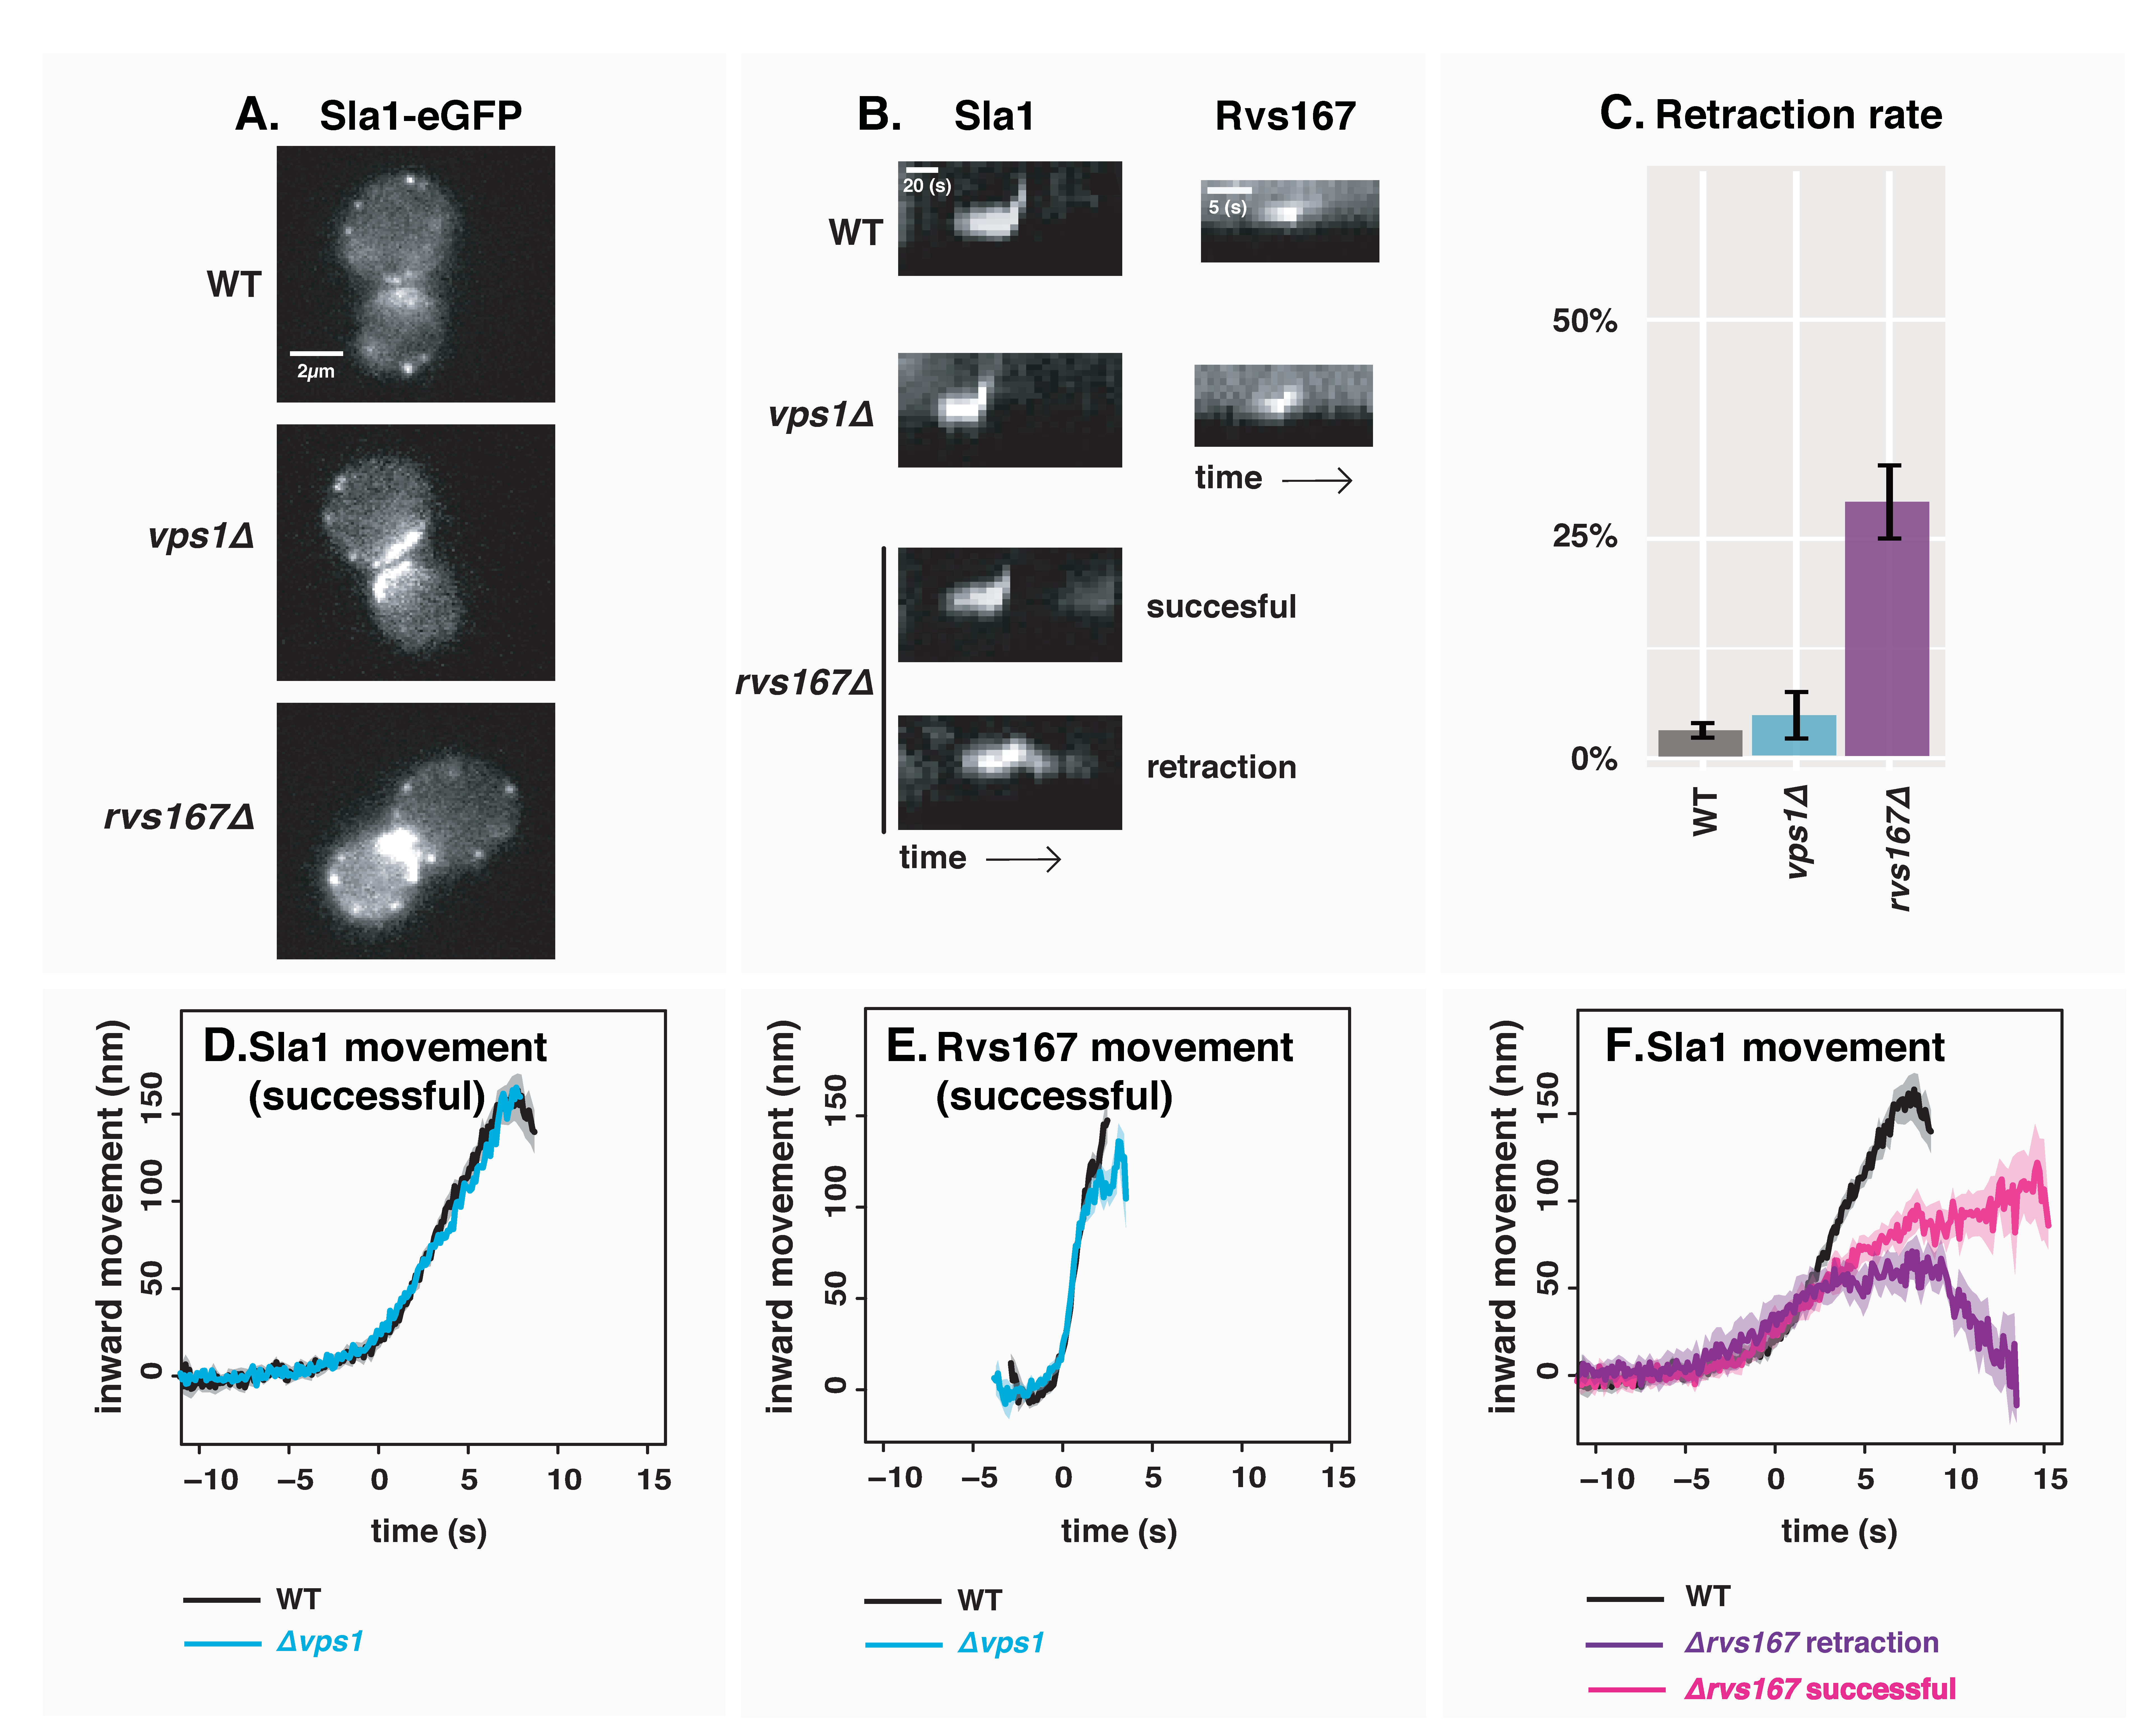
\includegraphics
	[width=0.97\hsize]{/Users/deepikaa/Desktop/scission_paper/figures/fig1/final/vpsdel_22.pdf}
	\caption{A: Slice of image of WT,  \textit{vps1$\Delta$}, and  \textit{rvs167$\Delta$} cells expressing Sla1-eGFP. Scale bar= 2{\textmu}m. B: Representative kymographs of Sla1-eGFP and Rvs167-eGFP patches in WT,  \textit{vps1$\Delta$}, and  \textit{rvs167$\Delta$} cells. Scale bar for Sla1-egfp = 20(s), scale bar for Rvs167-eGFP = 5(s). C: Histogram of Sla1-eGFP retraction percentages in WT,  \textit{vps1$\Delta$}, and  \textit{rvs167$\Delta$} cells. Error bars are standard deviation from two data sets, p<0.001 = *. D: Averaged centroid positions of Sla1-eGFP in WT and  \textit{vps1$\Delta$}  cells. E:  Averaged position of Rvs167-eGFP in WT and  \textit{vps1$\Delta$}  cells. F: Averaged position of Sla1-eGFP in WT, and successful and retracted Sla1-eGFP positions in \textit{rvs167$\Delta$} cells. All averaged positions are aligned in time to begin inward movement at the same time=0(s), and aligned in space to a starting position = 0(nm). Note that in E, averaged Rvs167-eGFP inward movement is concomitant with the maxima of its fluorescent intensity (Fig1.supplement3)} 
	\label{vps}
\end{figure}

To test whether absence of Vps1 influences scission, dynamics of endocytosis are observed in cells lacking Vps1 and compared against wild-type (WT) cells (Fig.\ref{vps}A-F). Vps1 deletion is confirmed by sequencing the open reading frame, and these cells show a growth phenotype at 37\si{\degree}C (Fig.1, supplement2) that has been previously reported (ref. ayscough). Rates of retraction of the membrane in \textit{vps1$\Delta$} and WT cells is quantified by tracking the endocytic coat protein Sla1 tagged at the C-terminus with eGFP (Fig.\ref{vps}C). Upon actin polymerization, the endocytic coat is pulled along with the membrane as it invaginates (ref.Skruzny?), and thus Sla1 acts as a proxy for the behaviour of the plasma membrane. Membrane retraction, that is, inward movement and subsequent retraction of the invaginated membrane back towards the cell wall is a scission-specific phenotype (ref.Marko). Retraction rates do not increase in  \textit{vps1$\Delta$} cells compared to the WT (Fig.\ref{vps}C). 

~\\

In order to study the total inward movement of the endocytic coat, and therefore the depth of the invagination, the centroid trajectory of ~50 Sla1-eGFP patches (ref. Picco, eLife 2015) in \textit{vps1$\Delta$} and WT cells is tracked and compared (Fig.\ref{vps}D). In brief, yeast cells expressing fluorescently-tagged endocytic proteins are imaged at the equatorial plane. Since membrane invagination progresses perpendicularly to the plane of the plasma membrane, proteins that move into the cytoplasm during invagination do so in the imaging plane. Centroids of 40-50 Sla1 patches- each patch being an endocytic site- are tracked in time and averaged. This provides an average centroid that can be followed with high spatial and temporal resolution. For more detail refer to Picco et. al, eLIFE 2015. Averaged centroid movement of Sla1-eGFP in WT cells is linear to about 140nm. Sla1 movement in \textit{vps1$\Delta$} cells has the same magnitude of movement (Fig.\ref{vps}D). In spite of slight differences in the rates of movement, the total inward movement- and so the depth of endocytic invagination- does not change. 
%When different endocytic proteins are simultaneously imaged with Actin Binding Protein Abp1, Abp1 provides a frame of reference to which all the other proteins can be aligned. Abp1 is used because it is abundant at endocytic sites and therefore easily imaged. Time=0 is established as the peak of the Abp1 fluorescence intensity in respective co-tagged strains strains. Abp1 fluorescent intensity maxima in wild-type cells is concomitant with the peak of Rvs167 fluorescent intensity and is time window in which scission occurs (ref2andrea, refwanda).  


~\\

Centroid tracking has shown that the number of molecules of Rvs167 peaks at the time of scission, and is followed by a rapid loss of fluorescent intensity, simultaneous with a sharp jump of the centroid into the cytoplasm (ref.Andrea). This jump, also seen in Rvs167-GFP kymographs (Fig.\ref{vps}B), is interpreted as loss of protein on the membrane tube, causing an apparent spatial jump to the protein localized at the base of the newly formed vesicle. Kymographs of Rvs167-GFP (Fig.\ref{vps}B), as well as Rvs167 centroid tracking (Fig.\ref{vps}E) in Vps1 deleted cells show the same jump. 

%Sla1 and Rvs167 behaviour in \textit{vps1$\Delta$} cells  indicate that loss of Vps1 does not influence the depth of membrane invagination or scission dynamics.
~\\

Since removal of the Rvs complex is known to increase the retraction rate at endocytic sites, involvement of the Rvs proteins in the scission process was investigated further. Rvs161 and Rvs167 form dimers (ref.Dominik), so deletion of Rvs167 effectively removes both proteins from endocytic sites. We quantified the effect of deletion of Rvs167 on membrane invagination (Fig.\ref{vps}A-C). 27\% of Sla1 patches that begin to form invaginations move inward and then retract in \textit{rvs167$\Delta$} cells (Fig.1C), consistent with retraction rates measured in other experiments (Kaksonen, Toret and Drubin, 2005), and suggesting failed scission in these 27\% of endocytic events. Coat movement of the retractions and of successful endocytic events were quantified (Fig.1F) as described in Picco et. al, 2015. Sla1 centroid movement in both successful and retracting endocytic events in \textit{rvs167$\Delta$} cells and WT look similar up to about 60nm (Fig.\ref{vps}F).  In successful endocytic events, Sla1-egfp signal is then lost, similar to WT cells, and Abp1 intensity drops (Fig.1supplement), indicating that scission occurs at invagination lengths between 60 -80 nm. That membrane scission occurs at shorter invagination lengths than in WT is corroborated by the smaller vesicles formed in \textit{rvs167$\Delta$} cells by Correlative light and electron microscopy (CLEM) (Kukulski et al., 2012). In retraction events, the Sla1 centroid moves back towards its original position. CLEM has also shown that Rvs167 localizes to endocytic sites after the invaginations are about 60nm long (Kukulski et al., 2012). Sla1 movement in \textit{rvs167$\Delta$}  indicates therefore that membrane invagination is unaffected till Rvs is supposed to arrive. 

%DISCUSSION?
%This indicates that first, membrane scission can occur at invagination lengths of 80nm. Then, that the arrival of Rvs prevents membrane scission at 80nm and allows further membrane invagination. In retraction events, after inward movement, the Sla1 centroid moves back towards the starting position, that is, to the plasma membrane. 



\subsection{Synaptojanins likely influence vesicle uncoating, but not scission dynamics.}

There are three Synaptojanin-like proteins in budding yeast: Inp51, Inp52, and Inp53 (Fig2a). Inp51-eGFP exhibits a diffuse cytoplasmic signal, and Inp53 localizes to patches within the cytoplasm- cellular localization that is consistent with involvement in trans-Golgi signalling (refGolgi)- Inp53 was not investigated further. Inp52-eGFP localizes to cortical actin patches that are endocytic sites (Fig2 supplement). Spatial and temporal alignment with Sla1 and Rvs167 shows that Inp52 protein molecules arrive in the late scission stage, and localizes to the bud tip, consistent with a role in membrane scission (Fig.2b). 

\begin{figure}
	\centering
	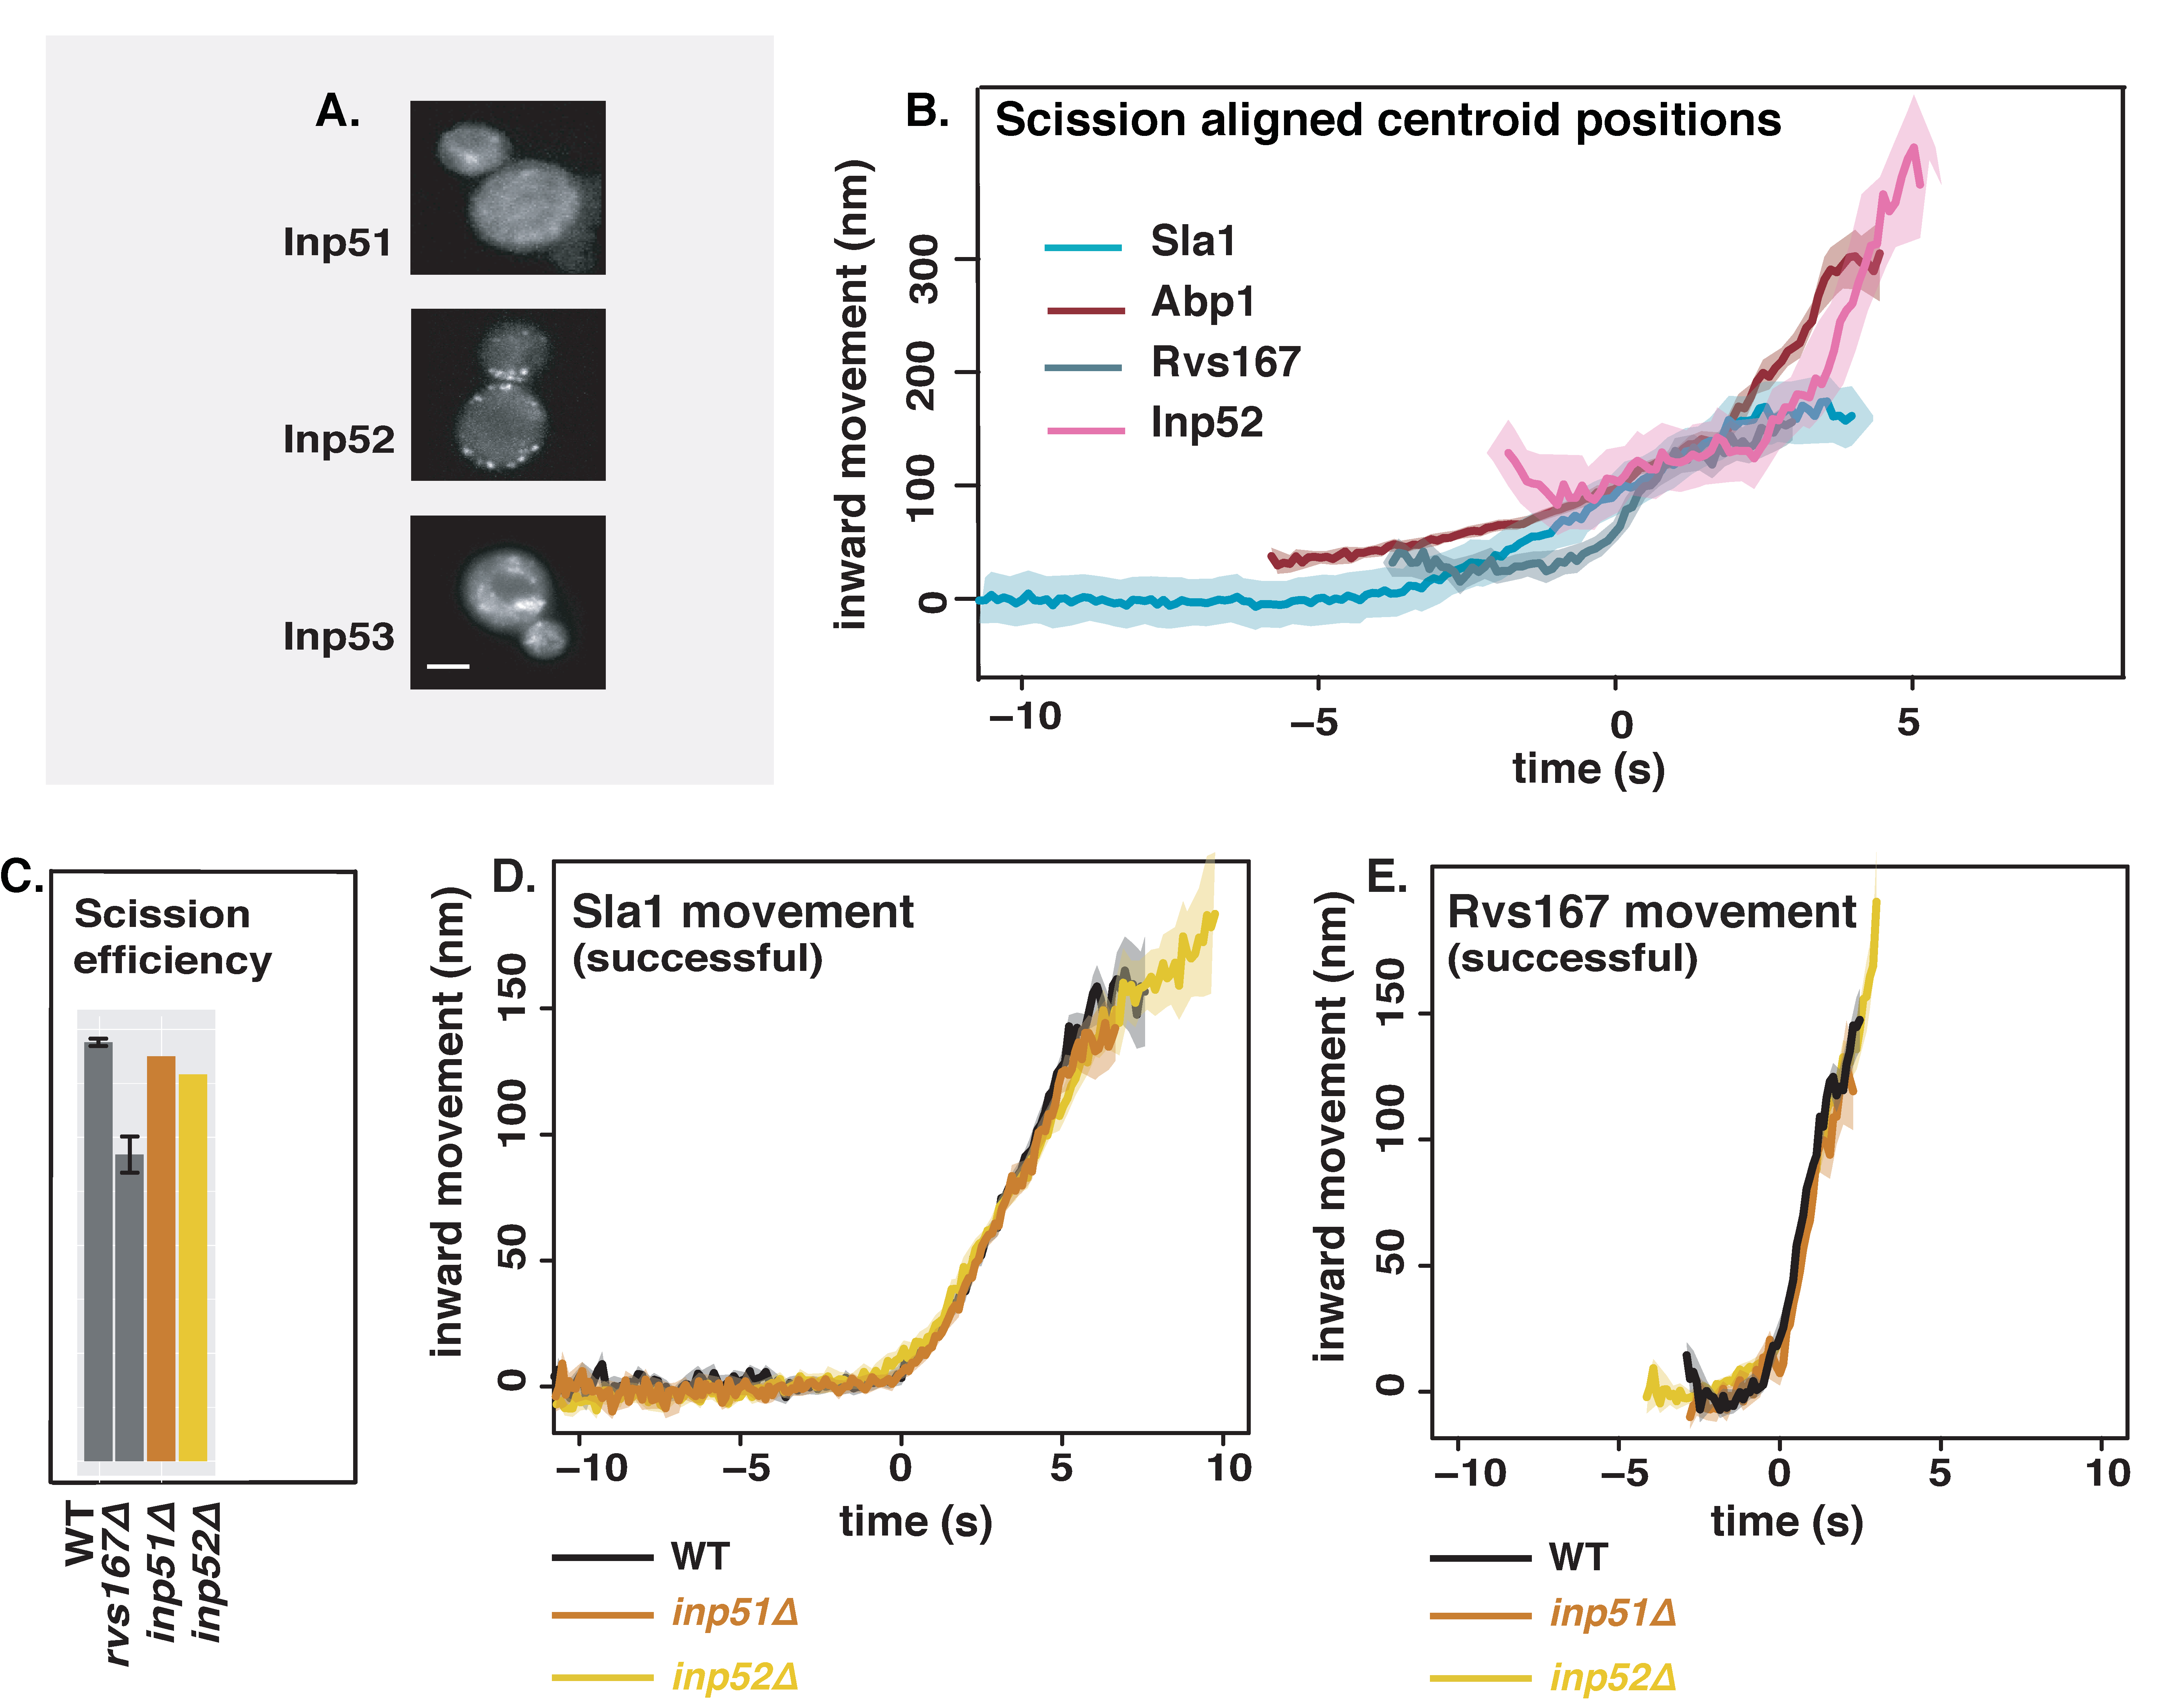
\includegraphics
	[width=0.8\hsize]{/Users/deepikaa/Desktop/scission_paper/figures/fig2/inp7.pdf}
	\caption{A half-columnwidth image using wrapfigure, to be used sparingly. Note that using a wrap figure before a sectional heading, near other floats or page boundaries is not recommended, as it may cause interesting layout issues. Use the optional argument to wrapfigure to control how many lines of text should be set half-width alongside it.}
	\label{fig:halfwidth}
\end{figure}


%INTRO?
%In mammalian cells, disruption of Synaptojanin genes results in cellular accumulation of PIP2 at endocytic sites. Coated vesicles gather at the plasma membrane, suggesting a role for lipid hydrolysis in releasing coat proteins from nascent vesicles (ref?). As an alternate to forces from Dynamin constriction, Liu et al (refliu) have proposed that an interaction between PiP2-hyrdolyzing Synaptojanins and BAR proteins could drive membrane scission. In this model Rvs BAR domains would form a scaffold on the membrane tube, preventing hydrolysis of underlying PIP2. Synaptojanin would arrive at inavaginated membranes, and hydrolyse unprotected PIP2. This generates a lipid boundary between BAR-protected PIP2 at the tube and hydrolyzed PIP2 at the bud tip. A line tension thus formed at the interphase between the two lipid types would then generate enough force to pinch off a vesicle.


Inp51 and Inp52 were tested as potential candidates for scission regulators. Sla1-eGFP and Rvs167-eGFP in cells with either Inp51 or  Inp52 deleted were studied. Retraction events do not significantly increase compared to the WT in either \textit{inp51$\Delta$} or \textit{inp52$\Delta$} cells (Fig2c). Magnitude and speed of coat movement in  \textit{inp51$\Delta$} is the same as the WT (Fig2.d). In  \textit{inp52$\Delta$} cells, coat movement also has the magnitude and speed as WT, but Sla1-eGFP signal is persistent after membrane scission (Fig.2d). Similarly, although Rvs167 inward movement looks the similar (Fig2e), disassembly has a delay, while the assembly is similar to WT (Fig2f). Assembly of Rvs167 has a delay in \textit{inp51$\Delta$} cells. The magnitude of the inward movement of both Sla1 and Rvs167 in cells containing either deletion are the same as in WT, while assembly and disassembly dynamics of Rvs167 is changed. 


%DISCUSSION
%This delay in decrease of Sla1-GFP signal is consistent with delay in vesicle uncoating rather than membrane scissison. 
%Rvs: Similarly, indicating a delay in removing endocytic proteins from the newly formed vesicle. Assembly of Rvs167 has a delay in \textit{inp51$\Delta$} cells , which could indicate a defect in recruiting proteins to endocytic sites, or in progression of endocytic invaginations. Since Sla1 movement is the same, we suggest a defect in the former rather than latter. 

%\begin{figure}
%			\hspace*{-1cm}
%				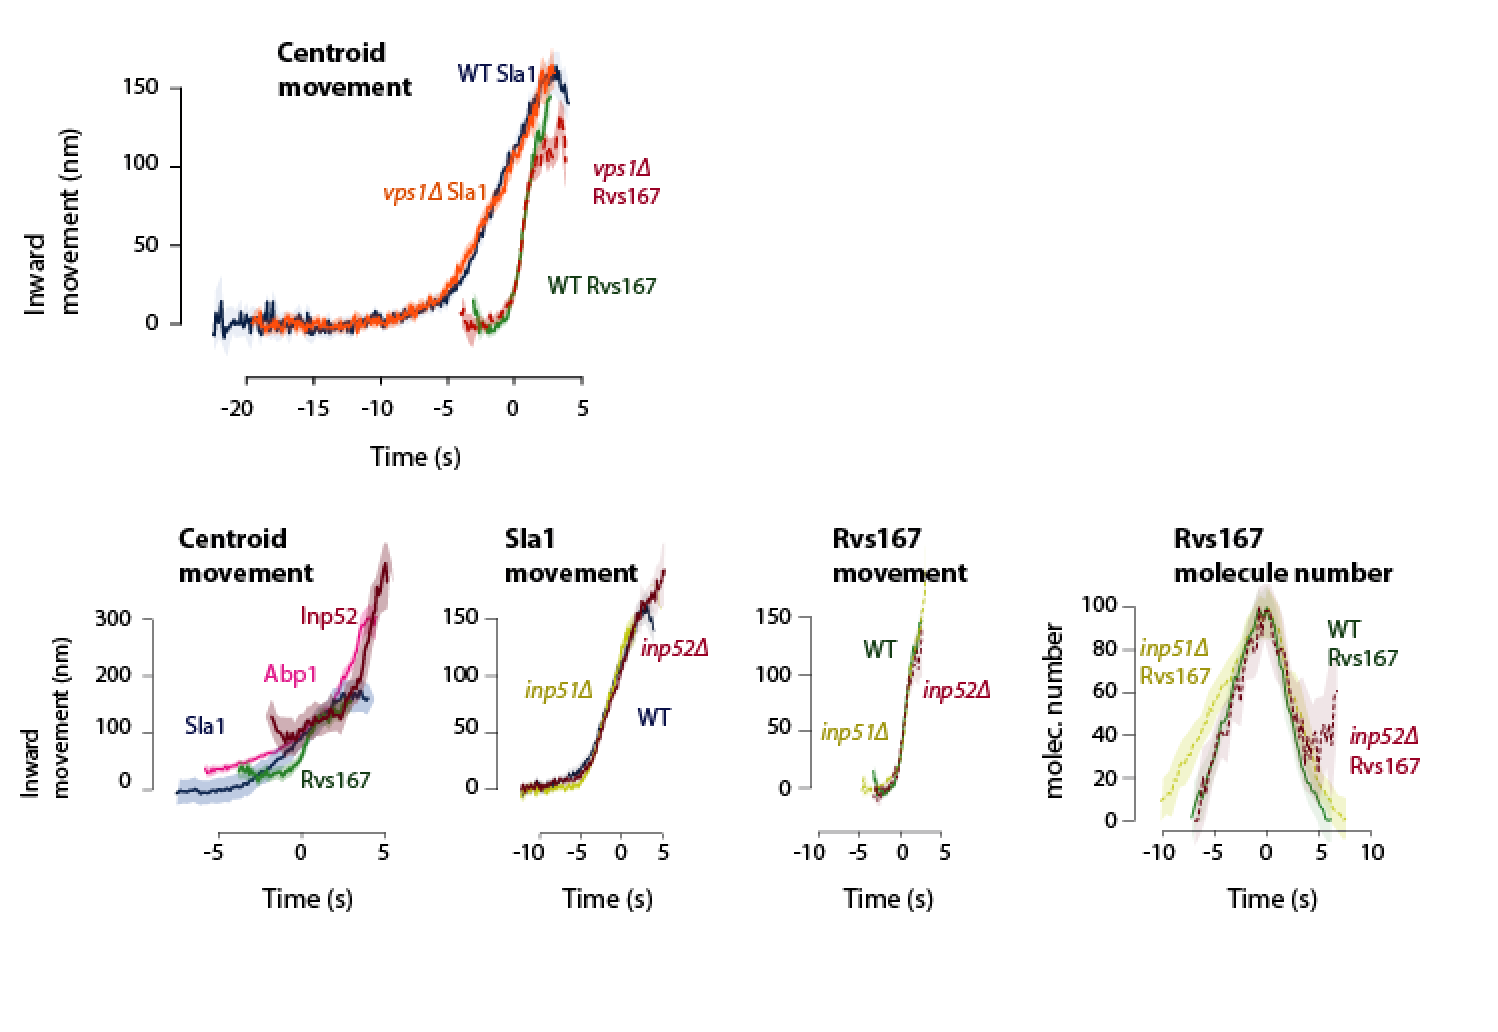
\includegraphics[width=4cm, height=4cm, keepaspectratio]{figures/vps1_placeholder}
%	\caption[Endocytic pathways in cells]
%			\label{intro_mayor}}
%\end{figure}

%\begin{wrapfigure}{l}{.46\textwidth}
%	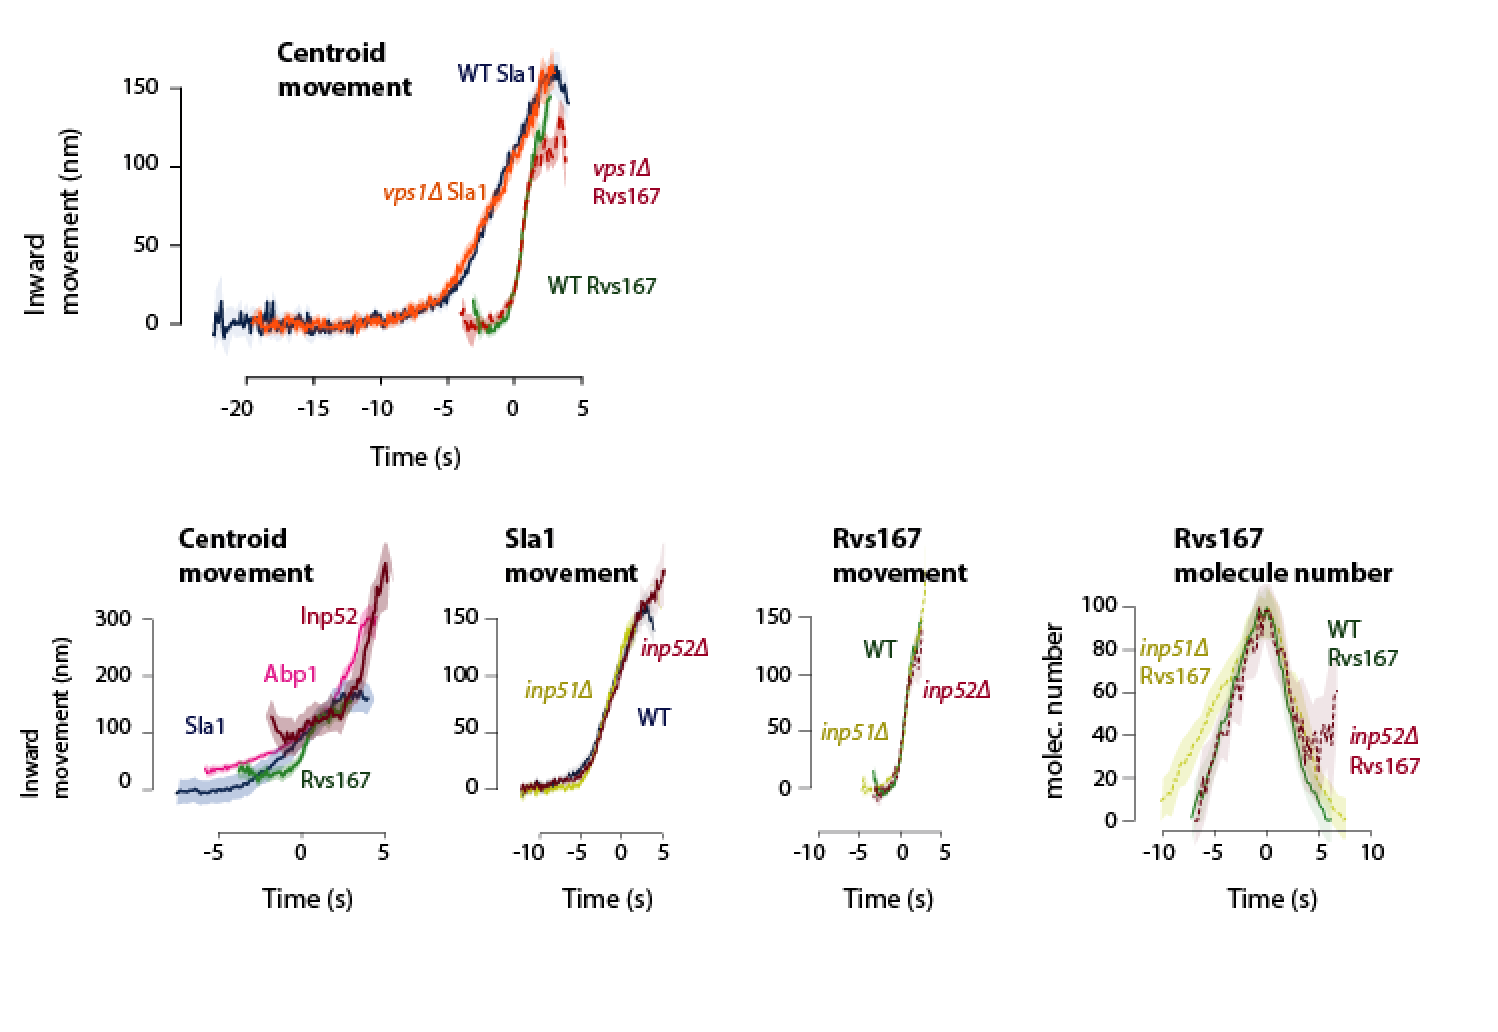
\includegraphics[width=\hsize]{figures/vps1_placeholder}
%	\caption{A half-columnwidth image using wrapfigure, to be used sparingly. Note that using a wrapfigure before a sectional heading, near other floats or page boundaries is not recommended, as it may cause interesting layout issues. Use the optional argument to wrapfigure to control how many lines of text should be set half-width alongside it.}
%	\label{fig:halfwidth}
%\end{wrapfigure}



\subsection{Rvs BAR domains recognize membrane curvature in-vivo}

\begin{figure}
	\centering
	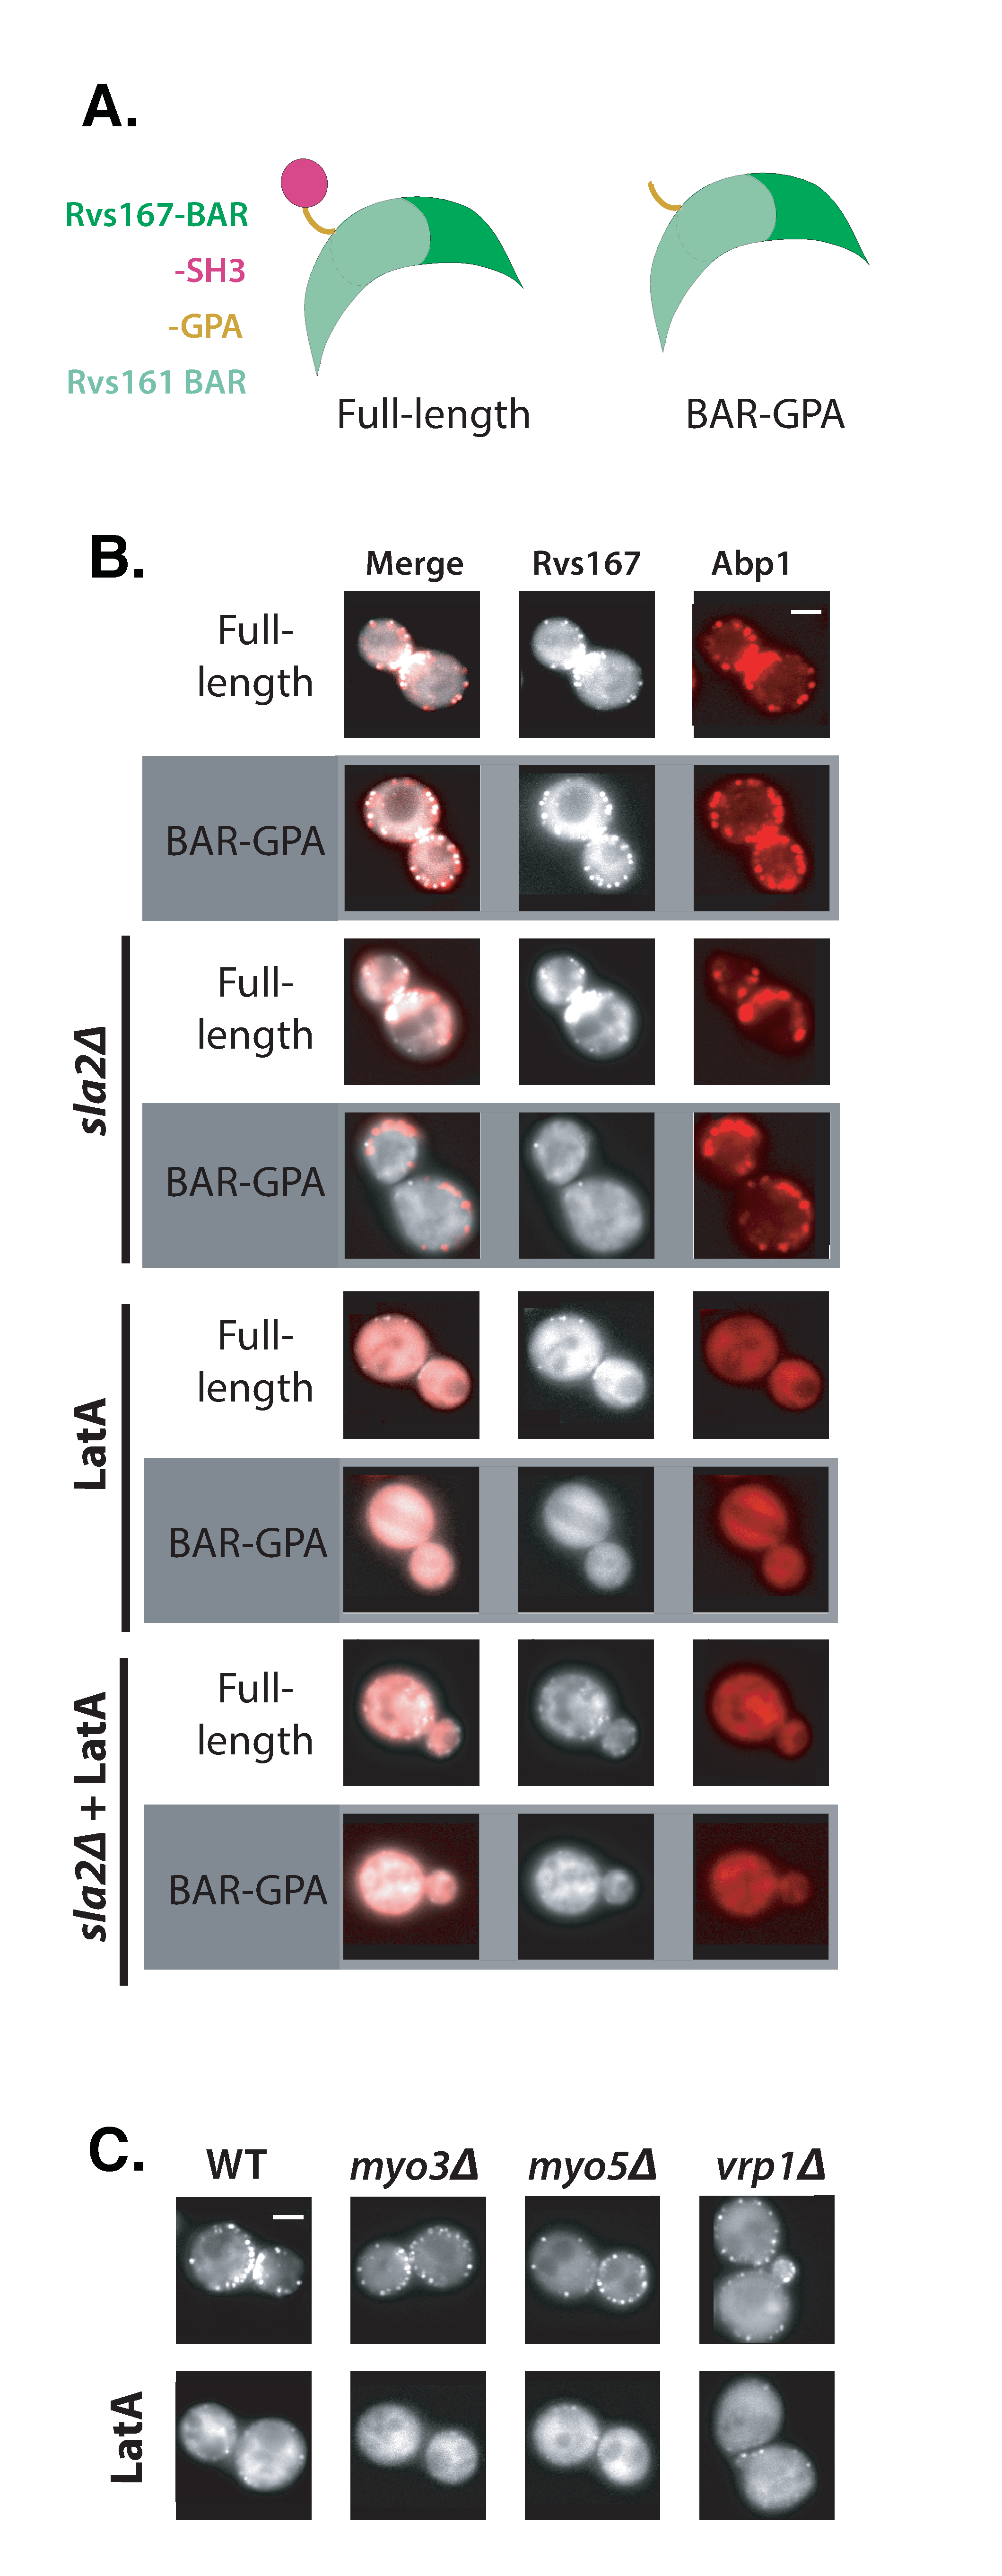
\includegraphics
	[width=0.6\hsize]{/Users/deepikaa/Desktop/scission_paper/figures/fig3/sla2_del_final12.pdf}
	\caption{A half-columnwidth image using wrapfigure, to be used sparingly. Note that using a wrap figure before a sectional heading, near other floats or page boundaries is not recommended, as it may cause interesting layout issues. Use the optional argument to wrapfigure to control how many lines of text should be set half-width alongside it.}
	\label{fig:halfwidth}
\end{figure}

%INTRO
%The curved tertiary structure and liposome binding assays of N-BAR domains have suggested that they may have a preference for curved membrane that match their own intrinsic curvature. Alternately, they may also impose their curvature on flat membrane and induce curvature formation. 

The interaction between Rvs167 and membrane curvature \textit{in vivo} has not so far been tested. In order to do so, we deleted the SH3 domain of Rvs167 leaving the N-terminal BAR region (henceforth BAR-GPA) and observed the localization of full-length Rvs167 and BAR-GPA (Fig3a). The GPA region is a disordered region that has no previously reported function and was retained to ensure proper folding and function of the BAR domain. Endogenously tagged Rvs167-eGFP and BAR-GPA-eGFP colocalization with Abp1-mCherry in WT and \textit{sla2$\Delta$} cells are compared (Fig3b). Sla2 acts as the molecular linker between forces exerted by the actin network and the plasma membrane (ref. Skruzny). \textit{sla2$\Delta$} cells therefore contain a polymerizing actin network at endocytic patches, but the membrane remains flat and endocytosis fails. In these cells, the full-length Rvs167 protein co-localizes with Abp1-mCherry, indicating that it is recruited to endocytic sites (Fig3b). BAR-GPA-eGFP localization is removed, except for rare transient patches that do not co-localize with Abp1-mCherry, indicating that in the absence of membrane curvature, the BAR domains  cannot localize to endocytic sites (Fig3b, \textit{sla2$\Delta$}). 


%DISCUSSION {Rvs SH3 domains contribute to curvature independent localization}
%We have shown that yeast N-BAR domains need membrane curvature to localize in vivo. Full-length Rvs167, however, is recruited to endocytic patches in \textit{sla2$\Delta$} cells. This indicates that a second interaction- that is not the BAR-curvature dependent- recruits the protein to endocytic sites. This interaction must come from the SH3 region, showing that Rvs localization is dependent on both BAR as well as SH3 domain interactions. Absence of the SH3 domain also reduces total recruitment of Rvs and Abp1 protein, giving the SH3 domain an important and surprising role in regulating the late stage of endocytosis. 

\subsection{SH3 domains are likely recruited by Myosin 3}
SH3 domains have been shown to interact with several proteins in the actin module of endocytosis. Type I myosins Myo3 and Myo5, and Vrp1 have genetic or physical interactions with Rvs167 SH3 domains (Lila and Drubin, 1997; Colwill et al., 1999, Madania et al., 1999; Liu et al., 2009). 
We tested the interaction between these proteins and the Rvs167-SH3 region by studying the localization of full-length Rvs167 in cells with one of these proteins deleted, and treated with LatA to reproduce the situation in which BAR-curvature interaction is removed, and SH3 interaction remains. 
Deletion of neither Vrp1 nor Myo5 in combination with LatA treatment removes the localization of Rvs167. Deletion of Myo3 with LatA treatment removes localization of Rvs167. 
\subsubsection{\color{red} 
	what about the differences in myo5 and myo3 number... 
}

\subsection{Loss of Rvs167 SH3 domain affects coat and actin dynamics}

\begin{figure}
	\centering
	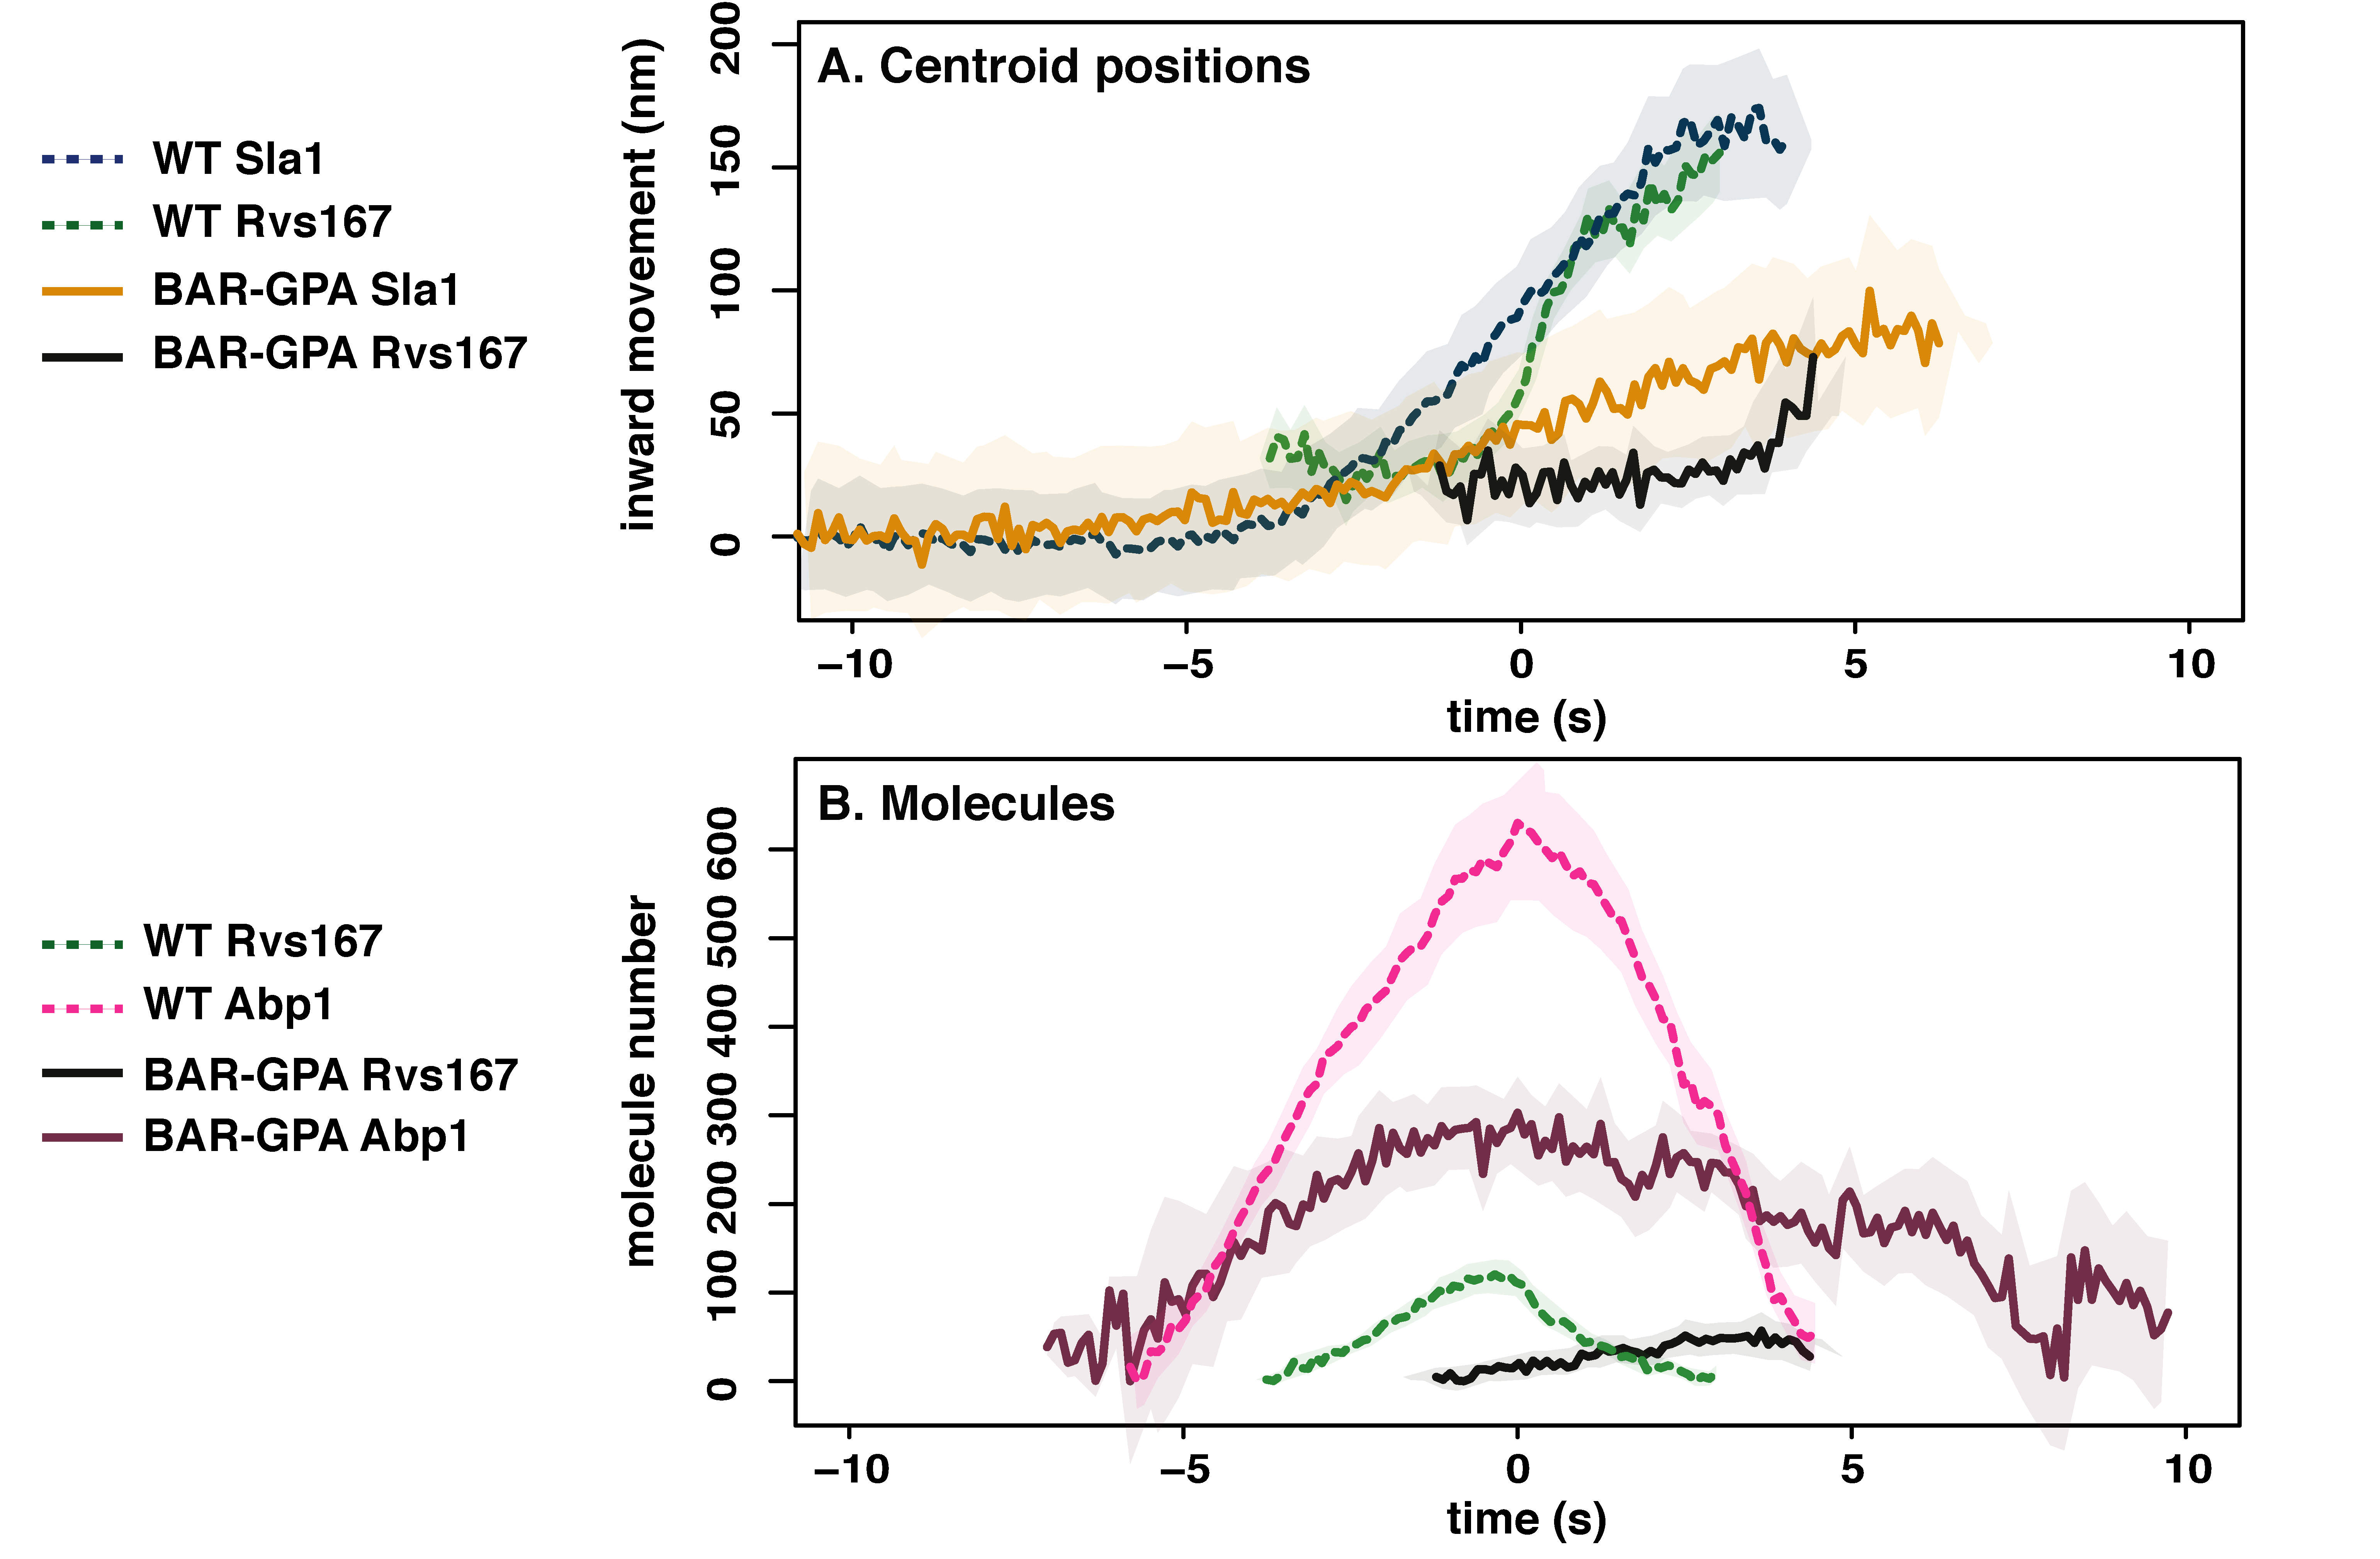
\includegraphics
	[scale=0.15]
	{/Users/deepikaa/Desktop/scission_paper/figures/fig4/delsh3_5.pdf}
	\caption{A half-columnwidth image using wrapfigure, to be used sparingly. Note that using a wrapfigure before a sectional heading, near other floats or page boundaries is not recommended, as it may cause interesting layout issues. Use the optional argument to wrapfigure to control how many lines of text should be set half-width alongside it.}
	\label{fig:halfwidth}
\end{figure}


In order to further probe the contribution of the Rvs167 SH3 domain to endocytosis, we compared dynamics of Sla1, as well as Rvs167 and BAR-GPA centroids (Fig4a). Movement of Sla1 centroid is reduced in BAR-GPA cells (Fig4a). Both full length Rvs167 and BAR-GPA however, arrive at endocytic coats when Sla1 centroid is about 30nm away from the initial position (Fig1a, red line to the y axis). Tubular invaginations are formed in BAR cells, and qualitatively resemble that in WT cells, as seen by CLEM (Fig.4 supplement). The inward jump of BAR-GPA is less than that of full-length Rvs167 (Fig.4b). Recruitment of BAR is reduced to half that of Rvs167 (Fig4c), although cytoplasmic concentration of Rvs167 and BAR are not different (Fig4 supplement). We also quantified the number of Abp1 and Rvs molecules recruited to endocytic sites (Fig4b). Abp1 disassembly is slowed down in BAR-GPA cells compared to WT (Fig4b), and recruitment is reduced to 50\% of WT recruitment (Fig.4c), likely indication disruption of actin network assembly. 
%This data shows that loss of the SH3 domain is detrimental to the progress of endocytic sites.

%To check if there was a change in the timing of endocytic progression, I quantified the lifetimes of BAR, Sla1 and Abp1 in BAR cells using total internal reflection fluorescence (TIRF) microscopy and compared these against WT Sla1, Abp1, and Rvs167. Unlike epifluorescence microscopy at the equatorial plane, in TIRF only fluorophores up to a depth of about 100nm from the glass-sample interphase are excited. This reduces fluorescent signal from the cytoplasm, allowing detection of low intensity fluorescent signal, and is a better method for quantification of protein lifetime than epifluorescence microscopy. Although this method is sensitive to low fluorescent intensity, as the proteins start to move inward into the cytoplasm, fluorescent intensity rapidly drops, because of the limited excitation depth. Therefore, rather than a quantification of the entire lifetime of the protein, this is a quantification of the non-motile lifetime of a protein that arrives at endocytic sites. Non-motile lifetimes of Rvs167, Bar, Sla1 and Abp1 are thus compared between cell type.

\subsection{N-helix and GPA domains do not contribute to recruitment of Rvs or membrane movement}
\lipsum[12]
	
\subsection{Reduced BAR domain recruitment corresponds to reduced membrane movement}
Decreased Sla1 movement in BAR-GPA cells (Fig4a) can be explained by loss of some interaction mediated by the SH3 domain, or because the BAR-GPA mutant is recruited in smaller numbers to endocytic sites. To check whether increasing the recruitment of the Rvs complex alone can rescue reduced Sla1 movement, Rvs167 and Rvs161 genes were duplicated endogenously (ref Huber) in diploid and haploid yeast cells. Diploid cells are thus generated containing either 4 copies of both Rvs genes (by gene duplication), 2 copies of each gene (WT diploid), or 1 copy (by deleting one copy of Rvs167 and Rvs161).  
In diploid cells (Fig5a-c), amount of Rvs167 recruited to sites increases with gene copy number (Fig5c). Adding excess Rvs to endocytic sites in the 4x case does not change the rate or total inward movement of  Sla1, or of Rvs167.
In the case of 1x Rvs, Sla1 movement is slightly reduced after 100nm (Fig5a). Magnitude of Rvs167 inward movement is unchanged, but the Rvs167-eGFP signal is lost immediately after the inward movement, unlike in the 4x and 2x cases. 
In haploid cells, increasing the number of Rvs167 and Rvs161 genes results in increased recruitment of Rvs167 to about 1.6 times the WT amount (Fig5f,h). Sla1 dynamics however, remains the same as in the WT(Fig5d). Duplicating the BAR-GPA domain alone rescues the loss of Sla1 movement in the 1x BAR-GPA, as well the inward jump of BAR-GPA itself (Fig5d,e). We measured the total number of Abp1 molecules at endocytic sites for different strains (Fig5g,h), and found that higher Abp1 numbers corresponds to larger Sla1 centroid movement. Total Abp1 numbers recruited are reduced for 1xBAR and  \textit{rvs167$\Delta$}  strains (Fig5g,h), suggesting a correlation between the maximum number of Abp1 recruited and total invagination length.




\begin{figure}[h]
	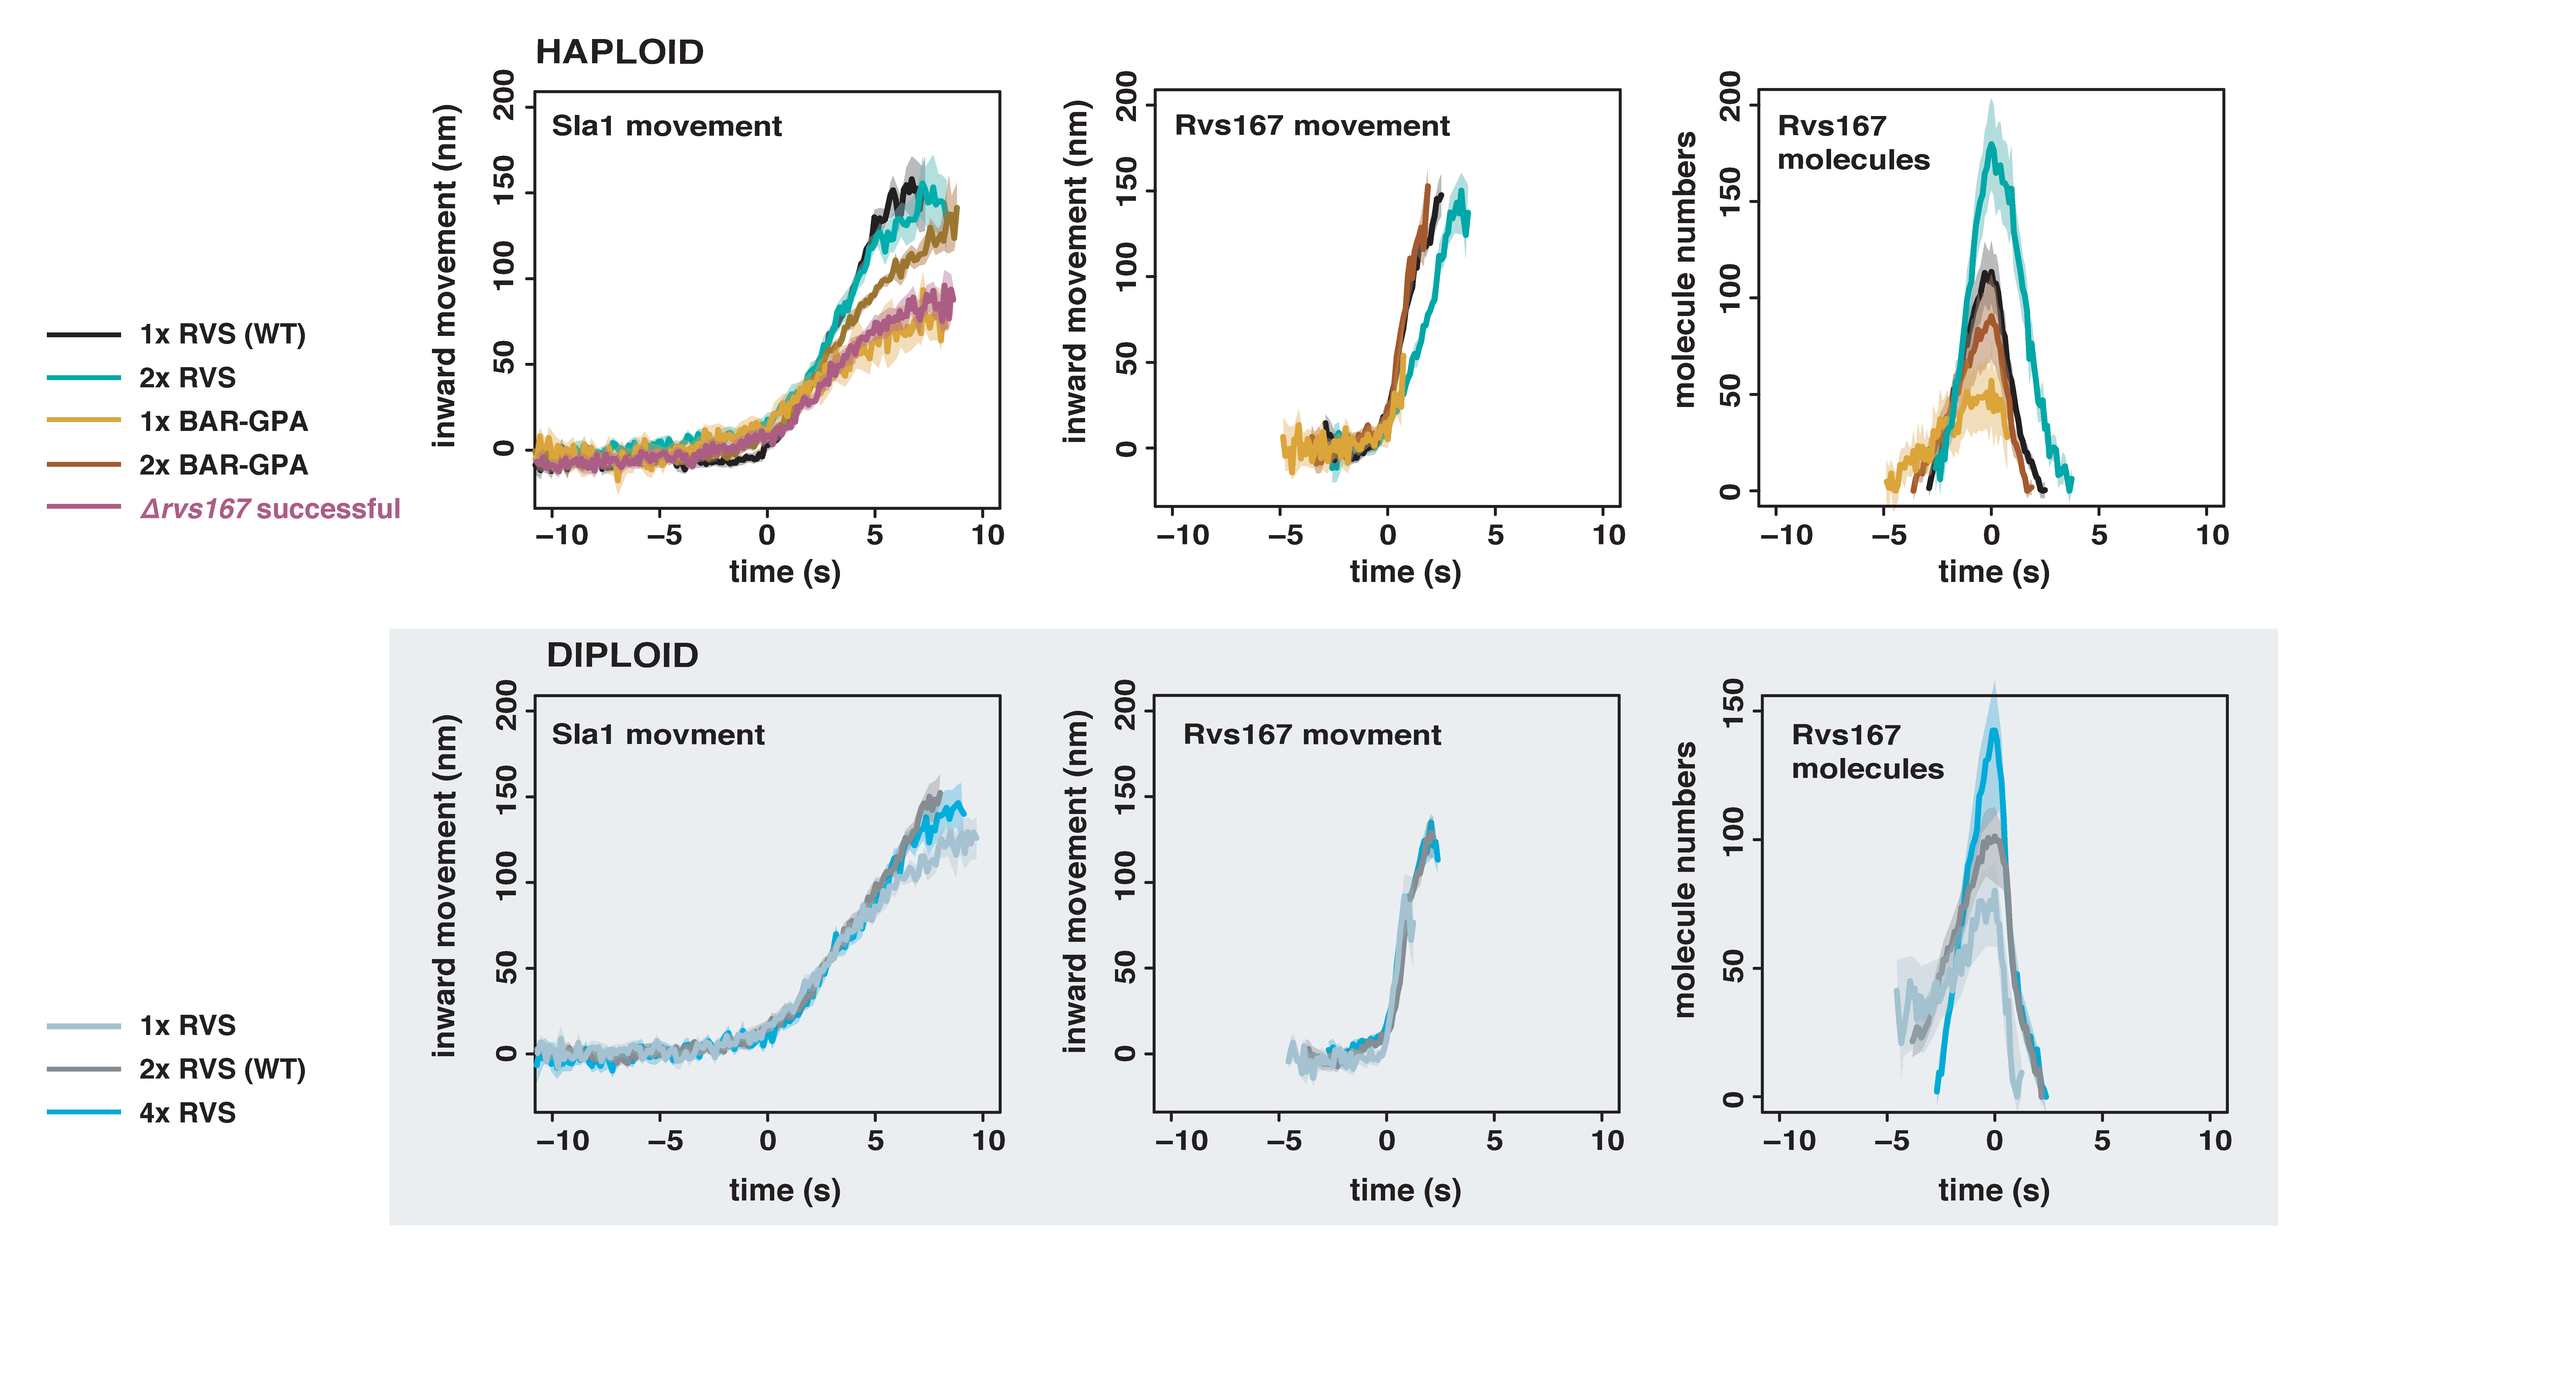
\includegraphics[
	width=1\textwidth,
	height=1\textwidth,
	keepaspectratio=true
	] {/Users/deepikaa/Desktop/scission_paper/figures/fig5/fig5_5.pdf}
	\caption{A half-columnwidth image using wrapfigure, to be used sparingly. Note that using a wrapfigure before a sectional heading, near other floats or page boundaries is not recommended, as it may cause interesting layout issues. Use the optional argument to wrapfigure to control how many lines of text should be set half-width alongside it.}
	\label{fig:halfwidth}
\end{figure}


%\begin{table}[bt]
%\caption{\label{tab:example}Automobile Land Speed Records (GR 5-10).}
% Use "S" column identifier to align on decimal point 
%\begin{tabular}{S l l l r}
%\toprule
%{Speed (mph)} & Driver          & Car                        & Engine    & Date     \\
%\midrule
%407.447     & Craig Breedlove & Spirit of America          & GE J47    & 8/5/63   \\
%413.199     & Tom Green       & Wingfoot Express           & WE J46    & 10/2/64  \\
%434.22      & Art Arfons      & Green Monster              & GE J79    & 10/5/64  \\
%468.719     & Craig Breedlove & Spirit of America          & GE J79    & 10/13/64 \\

%\end{tabular}

%\medskip 
%Source: \url{https://www.sedl.org/afterschool/toolkits/science/pdf/ast_sci_data_tables_sample.pdf}

%\tabledata{This is a description of a data source.}

%\end{table}


\section{Discussion}

Recruitment and function of the Rvs complex in has been explored in this work, as well as several models for how membrane scission could be effected in yeast endocytosis. We propose that Rvs is recruited to endocytic sites by interactions between the Rvs BAR domains and invaginated membrane, and that SH3 domain mediated protein-protein interactions are required for efficient recruitment of Rvs to sites. Arrival of Rvs on membrane tube scaffolds the membrane and prevents premature membrane scission. Effective scaffolding depends on recruitment of a critical number of Rvs molecules. Rvs is a relatively short-lived protein at endocytic sites. It is recruited only once membrane tube is formed (Kaksonen, Toret and Drubin, 2005; Kukulski et al., 2012; Picco et al., 2015). FCS measurements (Boeke et al., 2014) have shown that the cytosolic concentrations of Rvs167 and Rvs161 are high (354nM and 721nM respectively) compared to other endocytic proteins like Las17, Vrp1, Myo3, and Myo5 (80-240nM). In spite of this, relatively few numbers of Rvs are recruited to endocytic sites, suggesting that recruitment is tightly regulated. In the case of Rvs, both timing and efficiency appear crucial to its function, the question is what confers both.

\subsection{BAR domains sense \textit{in vivo} membrane curvature and time recruitment of Rvs}

%4.1.1 BAR domain senses membrane curvature
The curved structure of BAR dimers (Peter et al., 2004; Mim et al., 2012) has suggested that Rvs is recruited by its preference for some membrane shapes over others, supported by its arrival at curved membrane tubes. In the absence of membrane curvature, in  \textit{sla2$\Delta$}  cells, the BAR domain alone does not localize to cortical patches (Fig.3b,c). This demonstrates for the first time that the BAR domain does indeed sense and requires membrane curvature to localize to cortical patches. Work on BAR domains have proposed that electrostatic interactions at the concave surface and tips of the BAR domain structure mediate membrane binding (Qualmann, Koch and Kessels, 2011). Mutations in these lipid-binding surfaces would clarify the interaction with underlying lipids, and test if Rvs relies on similar interactions.
BAR is able to localize to endocytic sites, and has a similar lifetime in WT cells (Fig4b). However, time alignment with Abp1 shows that there is a delay in the recruitment of BAR-GPA compared to Abp1 arrival, compared to full-length Rvd167 (Fig4c). The delayed recruitment occurs because the invagination takes longer to reach a particular length: Sla1 moves inwards at a slower rate in BAR cells, and it takes longer for the membrane in BAR-GPA cells to reach the same length as Rvs167. Rvs167 arrives in BAR cells when Sla1 has moved inwards 25-30nm (dashed red lines in Fig.4a), which is also the distance Sla1 has moved when Rvs167 arrives in WT. By the time Sla1 has moved this distance, the membrane is already tubular (Kukulski et al., 2012; Picco et al., 2015), consistent with Rvs arrival at invaginated tubes. This suggests Rvs recruitment is timed to specific membrane invagination length- therefore to a specific membrane curvature- and that this timing is provided by the BAR domain.

%In Fig.3.3.3B we see that while the full-length Rvs167 arrives about 4 seconds after the arrival of Abp1, BAR arrives only 6 seconds after Abp1 arrives. There is a time delay between Abp1 recruitment and BAR arrival, compared to the arrival of full-length Rvs167, confirmed by the TIRF measurement in 3.3.3D. The delay in recruitment could occur because the membrane has not acquired the required invagination length or because the loss of the SH3 domain causes delayed recruitment. That the delayed recruitment occurs because the invagination takes longer to reach a particular length is supported by the fact that Sla1 moves inwards at a slower rate in BAR cells. It takes longer for the membrane in BAR cells to reach the same length as WT. Rvs167 arrives in BAR cells when Sla1 has moved inwards 25-30nm (dashed red lines in Fig.3.3.3A), which is also the distance Sla1 has moved when Rvs167 arrives in WT. By the time Sla1 has moved this distance, the membrane is already tubular (Kukulski et al., 2012; Picco et al., 2015), consistent with Rvs arrival at invaginated tubes. This suggests Rvs recruitment is timed to specific membrane invagination length- therefore to a specific membrane curvature- and that this timing is provided by the BAR domain.

\subsection{SH3 domains allow efficient and actin independent recruitment}

Rvs167 in BAR cells accumulates to about half the WT number (Fig.3c), even though the same cytoplasmic concentration is measured (supplement Fig3?), indicating that the SH3 domain increases the efficiency of recruitment of Rvs.  In \textit{sla2$\Delta$} cells, full-length Rvs can assemble on the membrane (Fig.3b,c). Since BAR domains alone do not localize to patches in \textit{sla2$\Delta$} cells, full-length localization must be mediated by the SH3 domain, supporting a role for the SH3 domain in increasing recruitment of Rvs by clustering protein molecules. That full-length Rvs167 is able to assemble and disassemble at cortical patches in \textit{sla2$\Delta$} cells without the curvature- dependent interaction of the BAR domain (Fig.3b,c) indicates that the SH3 domain is able to mediate both the recruitment and the disassembly of Rvs at the endocytic site. In \textit{sla2$\Delta$} cells treated with LatA (Fig.3c), actin-based membrane curvature is inhibited, and the actin patch proteins are removed from the plasma membrane. Full-length Rvs167 in these cells still shows transient localizations at the plasma membrane. In \textit{sla2$\Delta$} cells treated with LatA, the localization of BAR is lost. This suggests that localization of the full-length Rvs167 in LatA treated cells is dependent on an SH3 domain interaction, and that this is independent of both actin and membrane curvature.

In WT cells, the Abp1 and Rvs167 fluorescent intensities reach maxima concomitantly (Fig4b), and the consequent decay of both also coincide. Coincident disassembly indicates that upon vesicle scission, the actin network is immediately disassembled. Membrane scission essentially occurs around the intensity peak of the two proteins. This coincident peak is lost in BAR-GPA cells: BAR-GPA-eGFP in these cells peaks several seconds after Abp1 intensity starts to drop, and the decay of Abp1 is prolonged, taking nearly double the time as in WT. The number of Abp1 molecules recruited is decreased to about two thirds the WT number. Although it is not clear what the decoupling of Abp1 and Rvs peaks means, the changes in Abp1 dynamics suggests a strong disruption of the actin network dynamics. SH3 domains are known to interact with components of the actin network like Abp1 and Las17 (Lila and Drubin, 1997, Madania et al., 1999), but study of other components of the actin machinery will be required to understand how exactly loss of the SH3 has changed the progression of endocytosis.

SH3 interaction with an endocytic binding partner likely help recruit Rvs to endocytic sites. Many such interaction partners have been proposed. Abp1 interaction with the Rvs167 SH3 domain has been shown (Lila and Drubin, 1997; Colwill et al., 1999), as has one with WASP protein Las17 (Madania et al., 1999; Liu et al., 2009), yeast Calmodulin Cmd1 (Myers et al., 2016), type I myosins (Geli et al., 2000), and Vrp1 (Lila and Drubin, 1997). All of these suggested binding partners localize to the base of the invagination (Yidi Sun, 2006; Picco et al., 2015), and do not follow the invaginating membrane into the cytoplasm. The SH3 interaction partner is likely Myo3 (Fig3d), and SH3 domains interact with the endocytic network at the base of the invagination. Centroid tracking however, suggests that Rvs is accumulated all over the membrane tube. If Rvs was recruited to the base and pulled up as the invagination grows, the centroid would move continuously upwards rather than remain relatively non-motile before the jump at scission time. It is possible that the SH3 initially helps cluster near the base, and as the membrane invaginations grow longer, BAR-membrane interactions dominate.


\subsection{Accumulation of Rvs on membrane invagination}
When ploidy is doubled from haploid to diploid yeast cells, we could expect that double the protein amount is expressed and recruited, but it does not appear so. The amount of Rvs recruited in WT haploid  and diploids remains about the same, and cytoplasmic signal is similar (Fig.5, Fig5 supplement). This invariance between accumulated protein in haploids and diploids shows that Rvs recruitment is not determined by the number of alleles of Rvs. Haploid and diploid cells appear to tune the amount of Rvs recruitment to get a specific amount to endocytic sites.
WT diploids (2xd) contain two copies each of RVS161 and RVS167 genes. Rvs duplicated diploids, which contain four copies each of RVS167 and RVS161 (4xd) could be expected to express and recruit to sites twice the amount of Rvs as 2xd. However, compared to 2xd, cytoplasmic signal in 4xd increases by 1.6x and recruitment of Rvs167 to endocytic sites increases only by 1.4x. Doubling the gene copy number increases, but does not double protein expression or recruitment in the case of Rvs. Similarly, duplicating Rvs genes in haploid cells results in an increase in number of molecules recruited, but not in doubling (1xh, 2xh). Although the rate of adding Rvs is different in haploids and diploids, in both cases, it increases by gene copy number (yellow line in Fig.4.2).
Cytoplasmic protein concentration is increased when gene copy num- ber is increased, and recruitment to endocytic sites is increased by the increase in cytoplasmic concentration. These data suggest that the amount of Rvs that is recruited scales with available concentration of protein. Comparing across ploidy however, the rate of Rvs recruitment is lower in WT diploid compared to WT haploid (2xd vs 1xh, Fig.4.1)

for this is not clear.
4.2 Arrangement of Rvs dimers on the mem- brane
A homology model of the Rvs BAR dimer structure based on Am- phiphysin suggests that it has the concave structure typical for N- BAR domains. Rvs is a hetero- rather than homodimer unlike Am- phiphysin, and a high-resolution structure will be necessary to clarify the interaction and arrangement of Rvs on endocytic tubes. There are some indications from the experiments in this thesis however, regarding its interaction with the membrane.
4.2.1 Rvs does not form a tight scaffold on membrane tubes
Observations of in vitro helices of BAR domains have suggested that Rvs might form a similar helical scaffold. The number of Rvs molecules recruited to endocytic sites is high enough to cover the surface area of the tubular invagination, so it has been proposed that an Rvs scaffold covers the entire membrane tube up to the base of the future vesicle (Picco et al., 2015).
In Rvs duplicated diploid cells (4xd), Rvs can be recruited at a much faster rate than in the WT (2xd) (Fig.3.10B-C, Fig.4.2) while disassembly dynamics is the same in both (Fig.3.10C, Fig.4.3). The exponential decay of fluorescent intensity in WT haploid and diploid cells (1xh, 2xd, Fig.4.3) indicates that all of the protein is suddenly disassembled from the endocytic site. When the membrane tube undergoes scission, there is no more tubular curvature for the Rvs to bind to. The sharp decay is therefore consistent with a BAR scaffold that breaks upon vesicle scission because there is no more membrane interaction, releasing all the membrane-bound protein at once. A similar decay in the 4xd strain suggests that all the Rvs in this case is also bound to the membrane: if the protein was not bound to the membrane, fluorescent intensity would not decay sharply. Since the membrane is able to accommodate 1.4x the amount of BAR protein as the WT, it would suggest that at lower protein amounts, a tight helix that covers the entire tube is not likely. Adding molecules to a tube already completely covered by a scaffold would result in a change in Rvs assembly and disassembly dynamics.
Further, additional molecules would have to be added at the top or base of a tight scaffold. At the top, the radius of curvature is decreased compared to the tube since this is the rounded vesicle region. At the base, the plasma membrane is nearly flat, and the Rvs BAR domain is similarly unlikely to favour interactions here. Otherwise the scaffold would have to be disrupted to add new molecules, which would likely slow down recruitment rate rather than speed it up. Molecules could also be added concentric to an existing scaffold. However, the concave surface of Rvs is known to interact with lipids, and multiple layers of BAR domains on the membrane tube would probably not show the sudden disassembly seen here.
I assume that the membrane surface area does not change in the 4xd compared to 2xd from the identical movement of Sla1 in both cases (Fig.3.10A). It is possible that a wider tube is formed, which would increase the membrane surface area for BAR binding. This would, however, require the BAR domains to interact with a lower radius of curvature than in WT. This seems unlikely, and in the absence of any indication otherwise, I assume that the membrane tubes in all diploid and haploid cases have the same width.
4.2.2 A limit for how much Rvs can be recruited to the membrane
In the case of Rvs duplication in haploids (2xh), a change in disas- sembly dynamics is seen (Fig.3.9C, Fig.4.3). In 2xh, the maximum number of molecules recruited is 178±7.5 compared to the maximum of 113.505±5.2 in WT (1xh). This is means that nearly 1.6x the WT amount of protein is recruited to membrane tubes in in the 2xh case. The Rvs167 fluorescent intensity in 2xh shows a delay in disassembly. This suggests that the excess protein may not be directly on the mem- brane, since if the protein was membrane bound, when the membrane breaks, the protein must be released. The excess Rvs could either interact with the actin network via the SH3 domain, or interact with other Rvs dimers. By a similar argument as in 4.2.1 above, I do not expect that multiple layers of BAR domains are formed, and that the excess protein is recruited by the interaction of the SH3 domain.
Another explanation for the delayed disassembly is that at high concentrations of Rvs like in the 2xh case, a tight BAR scaffold is formed, and the BAR domains interact with adjacent BAR domains. When the membrane undergoes scission, the protein is no longer membrane-bound, but lateral interactions delay disassembly of the scaffold. Lateral interactions between neighbouring BAR dimers have been shown in the case of Endophilin (Mim et al., 2012). It is not currently clear where the Rvs molecules are added in the 2xh case: supperresolution microscopy could clarify whether it is added at the membrane tube.
Whatever the arrangement of the Rvs complex on the membrane, disassembly dynamics is changed in the case of 2xh, compared to the other haploid and diploid strains. Since the number of Rvs molecules is highest in this strain, this suggests that there is a limit to how much Rvs can assemble on the tube without altering interaction with the endocytic protein network. 4.2.3 Conclusions for Rvs localization
All of these data support the idea that Rvs recruitment rate and total numbers are determined by concentration of protein in the cell. The maximum number of molecules that can interact with the membrane is limited by the surface area of the invagination. Although more can be recruited, Rvs molecules over a certain threshold interact in a different way with endocytic sites, possibly via the SH3 domain. Timing of recruitment to sites is by curvature-recognition via the BAR domain, while efficiency of recruitment and interaction with the actin network is established via the SH3 domain. 4.3 What causes membrane scission?


\subsection{Rvs acts as a membrane scaffold preventing membrane scission}
Invaginations in \textit{rvs167$\Delta$} cells undergo scission at short invagination lengths of about 80nm (Fig.3.2), compared to the WT lengths of 140nm. This shows that first, enough forces are generated at 80nm to cause scission. Then, that Rvs167 is required at membrane tubes to prevent premature scission. Prevention of scission at short invagination lengths can be explained by Rvs stabilizing the membrane invagination via membrane interactions of the BAR domain (Boucrot et al., 2012; Dmitrieff and Nédélec, 2015). Rvs preventing membrane scission could also be explained by the SH3 domain mediating actin forces to the invagination neck: one can imagine that the SH3 domain somehow decouples actin forces from the neck, and that this delays scission. Since invagination lengths of rvs167à cells are increased towards WT by overexpression of the BAR domain alone (Fig.3.12A), I propose that localization of Rvs BAR domains to the membrane tube stabilizes the membrane. This allows deep invaginations to grow until actin polymerization produces enough forces to overcome this stabilization and sever the membrane. Stabilization of the membrane tube increases with increasing amounts of BAR domains recruited to the membrane tube (Fig.3.12). The requirement for Rvs scaffolding cannot be removed by reducing turgor pressure (Fig.3.13), suggesting that the function of the scaffold is not to counter turgor pressure. 
~\\ 

Scission efficiency decreases with decreased amounts of Rvs: in diploids, lowering the amount of Rvs by 20 molecules decreases scission efficiency to about 90\% from 97\%. This indicates that a particular coverage of the membrane tube is required for effective scaffolding by BAR domains. In support of this, in BAR strains, fewer numbers of Rvs are recruited, and scission efficiency is similarly reduced. At low concentrations of Rvs like in the 1xd cells, it is likeley that some membrane tubes recruit the critical number of Rvs, in which case the invaginations grow to near WT lengths. Over a certain amount of Rvs, adding more BAR domains does not increase the stability of the tube: in 4xd, the same amount of actin is recruited before scission as in the 2xd and 1xd strains.
If enough forces are generated at 80nm, why is scission efficiency decreased in \textit{rvs167$\Delta$} compared to WT? Forces from actin may be at a threshold when the invagination is at 80nm. There could be enough force to sever the membrane, but not enough to sever reliably. The Rvs scaffold then keeps the network growing to accumulate enough actin to reliably cause scission. Controlling membrane tube length could also be a way for the cell to control the size of the vesicles formed, and therefore the amount of cargo packed into the vesicle.


\subsection{What causes membrane scission?}
 We have tested several scission models that include a major role for the Rvs complex. The seemingly obvious solution to the scission problem is the action of a dynamin-like GTPase. If loss of the yeast Dynamin Vps1 prevented or delayed scission, the membrane would continue to invaginate longer than WT lengths, and Sla1 movements of over 140nm should be observed. Rvs centroid movement would likely also be affected: a bigger jump inwards could indicate that a longer membrane has been cut. That neither is seen in the behaviour of coat and scission markers indicates that even if Vps1 is recruited to endocytic sites, it is not necessary for Rvs localization or function, and is not necessary for scission. The Inp51, Inp52 data tests the lipid hydrolysis model, in which synaptojanins hydrolyze PIP2 molecules that are not covered by BAR domains, resulting in a boundary between hydrolyzed and non- hydroplyzed PIP2. This model predicts that interfacial forces generated at the lipid boundary causes scission (Liu et al., 2006). Inp51 is not seen in patches at the cellular cortex, but this could be because protein recruitment is below our detection threshold. Inp52 localizes to the top of invaginations right before scission, consistent with a role in vesicle formation (Fig.3.7D). Some predictions of the lipid hydrolysis model are inconsistent with our data, however.
First, vesicle scission is expected to occur at the interphase of the hydrolyzed and non-hydrolyzed lipid. Since the BAR scaffold covers the membrane tube, this interphase would be at the top of the area covered by Rvs. Kukulski et al., 2012 have shown that vesicles undergo scission at 1/3 the invagination length from the base: that is, vesicles generated by the lipid boundary would be smaller than have been measured. Second, removing forces generated by lipid hydrolysis by deleting synaptojanins should increase invagination lengths, since scission would be delayed or it would fail without those forces. Deletion of neither Inp51 nor Inp52 changes the invagination lengths: Sla1 movement does not increase. That the position of the vesicle formed is also unchanged compared to WT is indicated by the similar magnitude of the jump into the cytoplasm of the Rvs centroid.
There are some changes in the synaptojanin deletion strains (Fig.3.8). In \textit{inp51$\Delta$} cells, Rvs assembly is slightly slower than that in WT. Therefore, Inp51 could play a role in Rvs recruitment. In the \textit{inp52$\Delta$} strain, about 12\% of Sla1-GFP tracks retract, indicated that scission fails in those cases. Although this is low compared to the failed scission rate of \textit{rvs167$\Delta$}  cells (close to 30\%), this data could suggest a moderate influence of Inp52 on scission. Rvs centroid persists after scission for about a second longer in \textit{inp52$\Delta$}  cells than in WT, indicating that disassembly of Rvs on the base of the newly formed vesicle is delayed.
Inp52 is likely involved in vesicle un- coating
Deletion of synaptojanin-like Inp52 does not affect the movement of the invagination. In spite of this, Sla1 patches persist for longer after scission in the \textit{inp52$\Delta$}  than in WT cells, as does Rvs167, indicated by the arrows in Fig.3.8A,D. Persistence of both suggests that rather than the scission timepoint, post-scission disassembly of proteins from the vesicle is inhibited in \textit{inp52$\Delta$} cells. Inp52 then plays a role in recycling endocytic proteins from the vesicle to the plasma membrane. The slower assembly of Rvs in \textit{inp51$\Delta$} and the increase in coat retraction rates of \textit{inp52$\Delta$} could indicate that there is a slight effect on Rvs recruitment, and that lipid hydrolysis could play a small role in scission.

~\\
Protein-friction mediated membrane scission proposes that BAR domains induce a frictional force on the membrane, causing scission. In Rvs duplicated haploid cells (2xh), adding up to 1.6x the WT (1xh) amount of Rvs to membrane tubes does not affect the length at which the membrane undergoes scission (Fig.3.9). If more BAR domains were added to the membrane tube, frictional force generated as the membrane is pulled under it should increase, and the membrane should rupture faster. That is, membrane scission occurs as soon as WT forces are generated on the tube. Since BAR domains are added at a faster rate in the 2xh cells, these forces would be reached at shorter invagination lengths. In 2xh cells, WT amount of Rvs is recruited at about 1.8 seconds before maximum fluorescent intensity, but scission does not occur at this time. Instead, Rvs continues to accumulate, and the invagination continues to grow. In diploid strains, adding 1.4x the WT amount of Rvs in the 4x Rvs case also does not change length of membrane that undergoes scission. Therefore, protein friction due to Rvs does not appear to contribute significantly to membrane scission in yeast endocytosis. 

%In inp51àinp52à cells, Rvs is accumulated at patches, but majority of Rvs patches do not show the typical sharp jump into the cytoplasm. Membrane morphology is hugely aberrant in these cells, complicating interpretation of this data (Srinivasan et al., 1997). Electron mi- croscopy shows long, undulating membrane invaginations (Srinivasan et al., 1997). Fluorescence microscopy shows that multiple endocytic sites that are assembled and disassembled at these long invaginations, and fail to undergo scission (Sun et al., 2007). Where on these long membranes Rvs localizes could be clarified by CLEM or super- resolution microscopy. Large clusters of Rvs seen in the inp51àinp52à strain could be multiple Rvs patches on same membrane tube. Pooling signal from multiple endocytic sites would influence the molecule numbers acquired by our analysis, and yield a higher number than at a single site. Rvs does, interestingly, assemble and disassemble in these mutants. If no vesicles are formed at these membranes, it would indicate that Rvs disassembly is not caused by membrane scission.

Maximum amount of Abp1 measured in all the diploid strains is about 220 molecules (Fig.3.11). In this case, only one allele of Abp1 is fluorescently tagged, so half the amount of Abp1 recruited is measured. The maximum amount of Abp1 recruited is then double that measured, which is about 440±20 molecules (assuming equal expression and recruitment of tagged and untagged Abp1). In WT haploid cells, the maximum number of Abp1 measured is 460±20 molecules. That the same number of molecules of Abp1 is recruited in all cases before scission indicates that scission timing depends on the amount of Abp1, and hence, on the amount of actin recruited.
This data is consistent with actin supplying the forces necessary for membrane scission. The membrane invagination continues until the “right” amount of actin is recruited. At this amount of actin, enough forces are generated to rupture the membrane. The amount of force necessary is determined by the physical properties of the membrane like membrane rigidity, tension, and proteins accumulated on the membrane (Dmitrieff and Nédélec, 2015). Vesicle scission releases membrane-bound Rvs, resulting in release of the SH3 along with BAR domains. Release of the SH3 domains could indicate to its binding partner in the actin network that vesicle scission has occurred, beginning disassembly of actin components. In BAR strains, a low amount of actin is recruited (Fig.3.4C). Although the absence of the SH3 domain severely perturbs the actin network, the mechanistic effect of this perturbation is unclear.

\subsection{Model for membrane scission}
I propose that Rvs is recruited to sites by two distinct mechanisms. SH3 domains cluster Rvs at endocytic sites. This SH3 interaction increases the efficiency with which the BAR domains sense curvature on tubular membranes. BAR domains bind to endocytic sites by sensing tubular membrane. BAR domains are recruited over the entire membrane tube, but do not form a tight helical scaffold. Membrane shape is stabilized against fluctuations that could cause scission by the BAR-membrane interaction. This prevent actin forces from rupturing the membrane, and the invaginations continue to grow in length as actin continues to polymerize. BAR recruitment to membrane tubes is restricted by the surface area of the tube: after a certain amount of Rvs, the excess interacts with endocytic sites via the SH3 domain. Adding over a certain amount of Rvs also does not increase the stabilization effect on the tube. As actin continues to polymerize, at a certain amount of actin, enough forces are generated to overcome the resistance to membrane scission provided by the BAR scaffold. The membrane ruptures, and vesicles are formed. Synaptojanins may help recruit Rvs at endocytic sites: Inp51 and Inp52 have proline rich regions that could act as binding sites for Rvs167 SH3 domains. They are involved in vesicle uncoating post-scission, likely by dephosphorylating PIP2 and inducing disassembly of PIP2-binding endocytic proteins. Eventually phosphorylation regulation allows endocytic proteins to be reused at endocytic sites, while the vesicle is transported elsewhere into the cell.


%Fig.4C shows that recruitment of BAR is reduced to half that of Rvs167 (57±9.9 for BAR compared to 113.5±5.3 for Rvs167). Cytoplasmic concentration of Rvs167 and BAR are not different (supplement). The inward jump of BAR is less than that of full-length Rvs167 (Fig.4A). 
%DISCUSSIONThis indicates that although the BAR is expressed at the same level at WT Rvs167, it is recruited less efficiently. The inward jump of BAR is less than that of full-length Rvs167 (Fig.3.4A). The decrease in inward jump indicates that the position of the newly formed vesicle in BAR cells is lower than in WT. This would imply that invagination lengths are reduced in BAR cells compared to WT.
%We have shown that yeast N-BAR domains need membrane curvature to localize in vivo. Full-length Rvs167, however, is recruited to endocytic patches in \textit{sla2$\Delta$} cells. This indicates that a second interaction- that is not the BAR-curvature dependent- recruits the protein to endocytic sites. This interaction must come from the SH3 region, showing that Rvs localization is dependent on both BAR as well as SH3 domain interactions. Absence of the SH3 domain also reduces total recruitment of Rvs and Abp1 protein, giving the SH3 domain an important and surprising role in regulating the late stage of endocytosis. 

\lipsum[9]

\section{Methods and Materials}

Guidelines can be included for standard research article sections, such as this one. 

\lipsum[3]





\subsection{Citations}

LaTeX formats citations and references automatically using the bibliography records in your .bib file, which you can edit via the project menu. Use the \verb|\cite| command for an inline citation, like \cite{Aivazian917}, and the \verb|\citep| command for a citation in parentheses \citep{Aivazian917}. The LaTeX template uses a slightly-modified Vancouver bibliography style. If your manuscript is accepted, the eLife production team will re-format the references into the final published form. \emph{It is not necessary to attempt to format the reference list yourself to mirror the final published form.} Please also remember to \textbf{delete the line} \verb|\nocite{*}| in the template just before \verb|\bibliography{...}|; otherwise \emph{all} entries from your .bib file will be listed! 

%\begin{featurebox}
%\caption{This is an example feature box}
%\label{box:simple}
%This is a feature box. It floats!
%\medskip

%\includegraphics[width=5cm]{example-image}
%\featurefig{`Figure' and `table' captions in feature boxes should be entered with \texttt{\textbackslash featurefig} and \texttt{\textbackslash featuretable}. They're not really floats.}

%\lipsum[1]
%\end{featurebox}




\section{Acknowledgments}

Additional information can be given in the template, such as to not include funder information in the acknowledgments section.

\nocite{*} % This command displays all refs in the bib file. PLEASE DELETE IT BEFORE YOU SUBMIT YOUR MANUSCRIPT!
\bibliography{elife-sample}

%%%%%%%%%%%%%%%%%%%%%%%%%%%%%%%%%%%%%%%%%%%%%%%%%%%%%%%%%%%%
%%% APPENDICES
%%%%%%%%%%%%%%%%%%%%%%%%%%%%%%%%%%%%%%%%%%%%%%%%%%%%%%%%%%%%


\end{document}
